%	-------------------------------------------------------------------------------
% 
%
%
%
%
%
%
%
%
%
%	-------------------------------------------------------------------------------

	\documentclass[12pt, a4paper, oneside]{book}
%	\documentclass[12pt, a4paper, landscape, oneside]{book}

		% --------------------------------- 페이지 스타일 지정
		\usepackage{geometry}
%		\geometry{landscape=true	}
		\geometry{top 		=10em}
		\geometry{bottom		=10em}
		\geometry{left		=8em}
		\geometry{right		=8em}
		\geometry{headheight	=4em} % 머리말 설치 높이
		\geometry{headsep		=2em} % 머리말의 본문과의 띠우기 크기
		\geometry{footskip		=4em} % 꼬리말의 본문과의 띠우기 크기
% 		\geometry{showframe}
	
%		paperwidth 	= left + width + right (1)
%		paperheight 	= top + height + bottom (2)
%		width 		= textwidth (+ marginparsep + marginparwidth) (3)
%		height 		= textheight (+ headheight + headsep + footskip) (4)



		%	===================================================================
		%	package
		%	===================================================================
%			\usepackage[hangul]{kotex}				% 한글 사용
			\usepackage{kotex}					% 한글 사용
			\usepackage[unicode]{hyperref}			% 한글 하이퍼링크 사용

		% ------------------------------ 수학 수식
			\usepackage{amssymb,amsfonts,amsmath}	% 수학 수식 사용
			\usepackage{mathtools}				% amsmath 확장판

			\usepackage{scrextend}				% 
		

		% ------------------------------ LIST
			\usepackage{enumerate}			%
			\usepackage{enumitem}			%
			\usepackage{tablists}				%	수학문제의 보기 등을 표현하는데 사용
										%	tabenum


		% ------------------------------ table 
			\usepackage{longtable}			%
			\usepackage{tabularx}			%
			\usepackage{tabu}				%




		% ------------------------------ 
			\usepackage{setspace}			%
			\usepackage{booktabs}		% table
			\usepackage{color}			%
			\usepackage{multirow}			%
			\usepackage{boxedminipage}	% 미니 페이지
			\usepackage[pdftex]{graphicx}	% 그림 사용
			\usepackage[final]{pdfpages}		% pdf 사용
			\usepackage{framed}			% pdf 사용

			
			\usepackage{fix-cm}	
			\usepackage[english]{babel}

		%	=======================================================================================
		% 	tikz package
		% 	
		% 	--------------------------------- 	
			\usepackage{tikz}%
			\usetikzlibrary{arrows,positioning,shapes}
			\usetikzlibrary{mindmap,trees}			

		%	=======================================================================================
		% 	listing package
		% 	
		% 	--------------------------------- 	
			\usepackage{listings}



		% --------------------------------- 	page
			\usepackage{afterpage}		% 다음페이지가 나온면 어떻게 하라는 명령 정의 패키지
%			\usepackage{fullpage}			% 잘못 사용하면 다 흐트러짐 주의해서 사용
%			\usepackage{pdflscape}		% 
			\usepackage{lscape}			%	 


			\usepackage{blindtext}
	
		% --------------------------------- font 사용
			\usepackage{pifont}				%
			\usepackage{textcomp}
			\usepackage{gensymb}
			\usepackage{marvosym}



		% Package --------------------------------- 
			\usepackage{tablists}				%

		% Package --------------------------------- 
			\usepackage[framemethod=TikZ]{mdframed}				% md framed package
			\usepackage{smartdiagram}								% smart diagram package


		% Package ---------------------------------    연습문제 

			\usepackage{exsheets}				%

			\SetupExSheets{solution/print=true}
			\SetupExSheets{question/type=exam}
			\SetupExSheets[points]{name=point,name-plural=points}


		% --------------------------------- 페이지 스타일 지정

		\usepackage[Sonny]		{fncychap}

			\makeatletter
			\ChNameVar	{\Large\bf}
			\ChNumVar	{\Huge\bf}
			\ChTitleVar		{\Large\bf}
			\ChRuleWidth	{0.5pt}
			\makeatother

%		\usepackage[Lenny]		{fncychap}
%		\usepackage[Glenn]		{fncychap}
%		\usepackage[Conny]		{fncychap}
%		\usepackage[Rejne]		{fncychap}
%		\usepackage[Bjarne]	{fncychap}
%		\usepackage[Bjornstrup]{fncychap}

		\usepackage{fancyhdr}
		\pagestyle{fancy}
		\fancyhead{} % clear all fields
		\fancyhead[LO]{\footnotesize \leftmark}
		\fancyhead[RE]{\footnotesize \leftmark}
		\fancyfoot{} % clear all fields
		\fancyfoot[LE,RO]{\large \thepage}
		%\fancyfoot[CO,CE]{\empty}
		\renewcommand{\headrulewidth}{1.0pt}
		\renewcommand{\footrulewidth}{0.4pt}
	
	
	
		%	--------------------------------------------------------------------------------------- 
		% 	tritlesec package
		% 	
		% 	
		% 	------------------------------------------------------------------ section 스타일 지정
	
			\usepackage{titlesec}
		
		% 	----------------------------------------------------------------- section 글자 모양 설정
			\titleformat*{\section}					{\large\bfseries}
			\titleformat*{\subsection}				{\normalsize\bfseries}
			\titleformat*{\subsubsection}			{\normalsize\bfseries}
			\titleformat*{\paragraph}				{\normalsize\bfseries}
			\titleformat*{\subparagraph}				{\normalsize\bfseries}
	
		% 	----------------------------------------------------------------- section 번호 설정
			\renewcommand{\thepart}				{\arabic{part}.}
			\renewcommand{\thesection}				{\arabic{section}.}
			\renewcommand{\thesubsection}			{\thesection\arabic{subsection}.}
			\renewcommand{\thesubsubsection}		{\thesubsection\arabic{subsubsection}}
			\renewcommand\theparagraph 			{$\blacksquare$ \hspace{3pt}}

		% 	----------------------------------------------------------------- section 페이지 나누기 설정
			\let\stdsection\section
			\renewcommand\section{\newpage\stdsection}



		%	--------------------------------------------------------------------------------------- 
		% 	\titlespacing*{commandi} {left} {before-sep} {after-sep} [right-sep]		
		% 	left
		%	before-sep		:  수직 전 간격
		% 	after-sep	 	:  수직으로 후 간격
		%	right-sep

			\titlespacing*{\section} 			{0pt}{1.0em}{1.0em}
			\titlespacing*{\subsection}	  		{0ex}{1.0em}{1.0em}
			\titlespacing*{\subsubsection}		{0ex}{1.0em}{1.0em}
			\titlespacing*{\paragraph}			{0em}{1.5em}{1.0em}
			\titlespacing*{\subparagraph}		{4em}{1.0em}{1.0em}
	
		%	\titlespacing*{\section} 			{0pt}{0.0\baselineskip}{0.0\baselineskip}
		%	\titlespacing*{\subsection}	  		{0ex}{0.0\baselineskip}{0.0\baselineskip}
		%	\titlespacing*{\subsubsection}		{6ex}{0.0\baselineskip}{0.0\baselineskip}
		%	\titlespacing*{\paragraph}			{6pt}{0.0\baselineskip}{0.0\baselineskip}
	


		%	--------------------------------------------------------------------------------------- 
		% 	toc 설정  - table of contents
		% 	
		% 	
		% 	----------------------------------------------------------------  문서 기본 사항 설정
			\setcounter{secnumdepth}{5} 		% 문단 번호 깊이
			\setcounter{tocdepth}{3} 			% 문단 번호 깊이 - 목차 출력시 출력 범위

			\setlength{\parindent}{0cm} 		% 문서 들여 쓰기를 하지 않는다.


		%	--------------------------------------------------------------------------------------- 
		% 	mini toc 설정
		% 	
		% 	
		% 	--------------------------------------------------------- 장의 목차  minitoc package
			\usepackage{minitoc}

			\setcounter{minitocdepth}{1}    	%  Show until subsubsections in minitoc
%			\setlength{\mtcindent}{12pt} 	% default 24pt
			\setlength{\mtcindent}{24pt} 	% default 24pt

		% 	--------------------------------------------------------- part toc
		%	\setcounter{parttocdepth}{2} 	%  default
			\setcounter{parttocdepth}{0}
		%	\setlength{\ptcindent}{0em}		%  default  목차 내용 들여 쓰기
			\setlength{\ptcindent}{0em}         


		% 	--------------------------------------------------------- section toc

			\renewcommand{\ptcfont}{\normalsize\rm} 		%  default
			\renewcommand{\ptcCfont}{\normalsize\bf} 	%  default
			\renewcommand{\ptcSfont}{\normalsize\rm} 	%  default


		%	=======================================================================================
		% 	tocloft package
		% 	
		% 	------------------------------------------ 목차의 목차 번호와 목차 사이의 간격 조정
			\usepackage{tocloft}

		% 	------------------------------------------ 목차의 내어쓰기 즉 왼쪽 마진 설정
			\setlength{\cftsecindent}{2em}			%  section

		% 	------------------------------------------ 목차의 목차 번호와 목차 사이의 간격 조정
			\setlength{\cftsecnumwidth}{2em}		%  section





		%	=======================================================================================
		% 	flowchart  package
		% 	
		% 	------------------------------------------ 목차의 목차 번호와 목차 사이의 간격 조정
			\usepackage{flowchart}
			\usetikzlibrary{arrows}



		%	=======================================================================================
		% 	줄 간격 설정
		% 	
		% 	
		% 	--------------------------------- 	줄간격 설정
			\doublespace
%			\onehalfspace
%			\singlespace
		
		

	% 	============================================================================== itemi Global setting

	
		%	-------------------------------------------------------------------------------
		%		Vertical spacing
		%	-------------------------------------------------------------------------------
			\setlist[itemize]{topsep=0.0em}			% 상단의 여유치
			\setlist[itemize]{partopsep=0.0em}			% 
			\setlist[itemize]{parsep=0.0em}			% 
%			\setlist[itemize]{itemsep=0.0em}			% 
			\setlist[itemize]{noitemsep}				% 
			
		%	-------------------------------------------------------------------------------
		%		Horizontal spacing
		%	-------------------------------------------------------------------------------
			\setlist[itemize]{labelwidth=1em}			%  라벨의 표시 폭
			\setlist[itemize]{leftmargin=8em}			%  본문 까지의 왼쪽 여백  - 4em
			\setlist[itemize]{labelsep=3em} 			%  본문에서 라벨까지의 거리 -  3em
			\setlist[itemize]{rightmargin=0em}			% 오른쪽 여백  - 4em
			\setlist[itemize]{itemindent=0em} 			% 점 내민 거리 label sep 과 같은면 점위치 까지 내민다
			\setlist[itemize]{listparindent=3em}		% 본문 드려쓰기 간격
	
	
			\setlist[itemize]{ topsep=0.0em, 			%  상단의 여유치
						partopsep=0.0em, 		%  
						parsep=0.0em, 
						itemsep=0.0em, 
						labelwidth=1em, 
						leftmargin=2.5em,
						labelsep=2em,			%  본문에서 라벨 까지의 거리
						rightmargin=0em,		% 오른쪽 여백  - 4em
						itemindent=0em, 		% 점 내민 거리 label sep 과 같은면 점위치 까지 내민다
						listparindent=0em}		% 본문 드려쓰기 간격
	
%			\begin{itemize}
	





% ------------------------------------------------------------------------------
% Begin document (Content goes below)
% ------------------------------------------------------------------------------
	\begin{document}
	
			\dominitoc
			\doparttoc			




			\title{TikZ 연습}
			\maketitle


			\tableofcontents 		% 목차 출력
%			\listoffigures 			% 그림 목차 출력
			\cleardoublepage
			\listoftables 			% 표 목차 출력

% 	==============================================================================  style


		\mdfdefinestyle	{code_document} {
						outerlinewidth		=1pt			,%
						innerlinewidth		=2pt			,%
						outerlinecolor		=blue!70!black	,%
						innerlinecolor		=white 			,%
						roundcorner			=4pt			,%
						skipabove			=1.0em 			,%
						skipbelow			=1.0em 			,%
						leftmargin			=0em			,%
						rightmargin			=0em			,%
						innertopmargin		=1em 			,%
						innerbottommargin 	=1em 			,%
						innerleftmargin		=1em 			,%
						innerrightmargin	=1em 			,%
						backgroundcolor		=gray!4			,%
						frametitlerule		=true 			,%
						frametitlerulecolor	=white			,%
						frametitlebackgroundcolor=gray		,%
						frametitleaboveskip=0.4em 			,%
						frametitlebelowskip=0.4em 			,%
						frametitlefontcolor=white 			,%
						}



% 	==============================================================================  chapter  Flow chart
	\chapter{Tikz 기본 설정}
	\minitoc				% Creating an actual minitoc


%	-----------------------------------------------------------  section  
	\section{Tikz 사용 용지 설정}

		\paragraph{사용 용지 설정}

			\begin{small}
			\begin{verbatim}
				\usepackage{geometry}
				\geometry{top       =10em}
				\geometry{bottom  =10em}
				\geometry{left        =8em}
				\geometry{right      =8em}
				\geometry{headheight  =4em} % 머리말 설치 높이
				\geometry{headsep     =2em} % 머리말의 본문과의 띠우기 크기
				\geometry{footskip     =4em} % 꼬리말의 본문과의 띠우기 크기
				
		%		paperwidth 	= left + width + right (1)
		%		paperheight 	= top + height + bottom (2)
		%		width 		= textwidth (+ marginparsep + marginparwidth) (3)
		%		height 		= textheight (+ headheight + headsep + footskip) (4)
			\end{verbatim}
			\end{small}
	



%	-----------------------------------------------------------  section  
	\section{Tikz set}


%	-----------------------------------------------------------  section  
	\section{Tikz style}



% 	==============================================================================  chapter  Flow chart
	\addtocontents{toc}{\protect\newpage}
	\chapter{기본 도형 그리기}
	\clearpage
	\minitoc				% Creating an actual minitoc
	

%	-----------------------------------------------------------  section  
	\section{기본 도형 그리기}


		\paragraph{color}

			\begin{itemize}
			\item	red
			\item	green
			\item	blue
			\item	cyan
			\item	brown
			\item	yellow
			\item	black
			\item	gray
			\item	white
			\end{itemize}

		\paragraph{line width}

			\begin{itemize}
			\item	ultra thick
			\item	very thick
			\item	thick
			\item	semithick
			\item	thin
			\item	very thin
			\item	ultra thin
			\item	line width=
			\end{itemize}


%	-----------------------------------------------------------  section    그리드
	\section{grid}


		\paragraph{grid - help line style} 	

			\tikzset{help lines/.style={ultra thin, blue!30}};
	%	------------------------------------------------ code	
		\begin{mdframed}[style=code_document, frametitle={code}]
			\begin{verbatim}
			\tikzset{help lines/.style={ultra thin, blue!30}};
			\end{verbatim}
		\end{mdframed}


		\paragraph{grid - gray} 	
			\tikz {\draw[line width=1pt, dashed, gray] (0,0) grid (6,6) }

	%	------------------------------------------------ code	
		\begin{mdframed}[style=code_document, frametitle={code}]
			\begin{verbatim}
			\tikz {\draw	[line width=1pt, dashed, gray] 
						(0,0) grid (6,6) }
			\end{verbatim}
		\end{mdframed}

		\paragraph{grid - black} 	
			\tikzset{help lines/.style={ultra thin, blue!30}};
			\tikz {\draw[line width=1pt, dashed, black] (0,0) grid (6,6) }
			
	%	------------------------------------------------ code	
		\begin{mdframed}[style=code_document, frametitle={code}]
			\begin{verbatim}
			\tikzset{help lines/.style={ultra thin, blue!30}};
			\tikz {\draw	[line width=1pt, dashed, black] 
						(0,0) grid (6,6) }
			\end{verbatim}
		\end{mdframed}


		\clearpage
		\paragraph{Grid}
			
\begin{tikzpicture}
			\draw[step=1cm,black,very thin] (-2,-2) grid (6,6);
			\end{tikzpicture}

	%	------------------------------------------------ code	
		\begin{mdframed}[style=code_document, frametitle={code}]
			\begin{verbatim}
			
\begin{tikzpicture}
			\draw	[step=1cm,black,very thin] 
					(-2,-2) grid (6,6);
			\end{tikzpicture}
			\end{verbatim}
		\end{mdframed}
	
		\paragraph{Grid - 테두리 삭제}
			\begin{tikzpicture}
			\draw[step=1cm,black,very thin] (-1.9,-1.9) grid (5.9,5.9);
			\end{tikzpicture}

	%	------------------------------------------------ code	
		\begin{mdframed}[style=code_document, frametitle={code}]
			\begin{verbatim}
			\begin{tikzpicture}
			\draw	[step=1cm,black,very thin] 
					(-1.9,-1.9) grid (5.9,5.9);
			\end{tikzpicture}
			\end{verbatim}
		\end{mdframed}

		\clearpage			
		\paragraph{Grid - line}

			\tikz\draw[line width=0.1pt, gray!30] (0,0) grid (3,2);
			\tikz\draw[line width=0.1pt, gray!30, step=10mm] (0,0) grid (3,2);
			\tikz\draw[line width=0.1pt, gray!30, step=5mm] (0,0) grid (3,2);

	%	------------------------------------------------ code	
		\begin{mdframed}[style=code_document, frametitle={code}]
			\begin{verbatim}
			\tikz\draw	[line width=0.1pt, gray!30] 
						(0,0) grid (3,2);
			\tikz\draw	[line width=0.1pt, gray!30, step=10mm] 
						(0,0) grid (3,2);
			\tikz\draw	[line width=0.1pt, gray!30, step=5mm] 
						(0,0) grid (3,2);
			\end{verbatim}
		\end{mdframed}


		\paragraph{Grid - Help lines}
			\tikz\draw	[help lines] 
						(0,0) grid (3,2);
			\tikz\draw	[help lines, gray!30] 
						(0,0) grid (3,2);
			\tikz\draw	[help lines, gray!30, step=2mm] 
						(0,0) grid (3,2);

	%	------------------------------------------------ code	
		\begin{mdframed}[style=code_document, frametitle={code}]
			\begin{verbatim}
			\tikz\draw	[help lines] 
						(0,0) grid (3,2);
			\tikz\draw	[help lines, gray!30] 
						(0,0) grid (3,2);
			\tikz\draw	[help lines, gray!30, step=2mm] 
						(0,0) grid (3,2);
			\end{verbatim}
		\end{mdframed}


%	-----------------------------------------------------------  section    축 과 마크
	\section{coordinate Labels}
	
	
		\paragraph{coordinate Labels - path}
	
	
			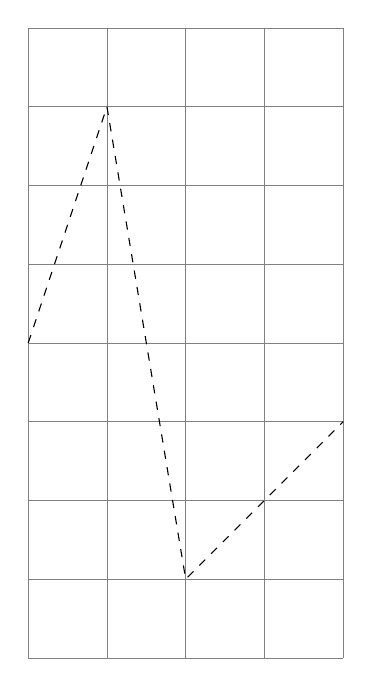
\begin{tikzpicture}
			\draw	[help lines] (-2,-4) grid (+2,+4);
			\path 	(-2,+0) coordinate (c1)
				 	(-1,+3) coordinate (c2)
				 	(+0,-3) coordinate (c3)
				 	(+2,-1) coordinate (c4);
			\draw 	[dashed]
					(c1) -- (c2) -- (c3)  -- (c4);	 	
			\end{tikzpicture}

	%	------------------------------------------------ code	
		\begin{mdframed}[style=code_document, frametitle={code}]
			\begin{verbatim}
			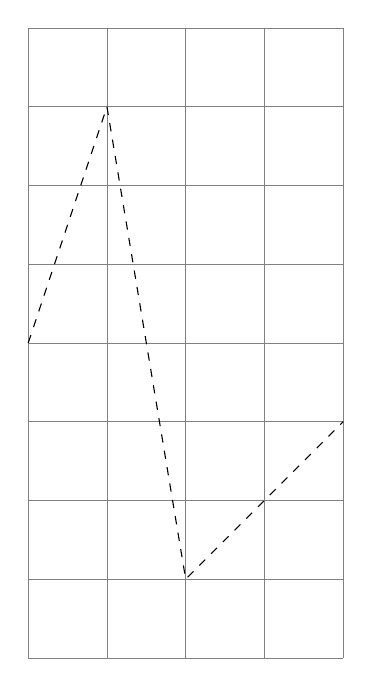
\begin{tikzpicture}
			\draw	[help lines] (-2,-4) grid (+2,+4);
			\path 	(-2,+0) coordinate (c1)
				 	(-1,+3) coordinate (c2)
				 	(+0,-3) coordinate (c3)
				 	(+2,-1) coordinate (c4);
			\draw 	[dashed]
					(c1) -- (c2) -- (c3)  -- (c4);	 	
			\end{tikzpicture}
			\end{verbatim}
		\end{mdframed}



%	-----------------------------------------------------------  section    축 과 마크
	\section{cycle Operation - 닫힌 도형을 만든다}

		\paragraph{cycle Operation}
	
			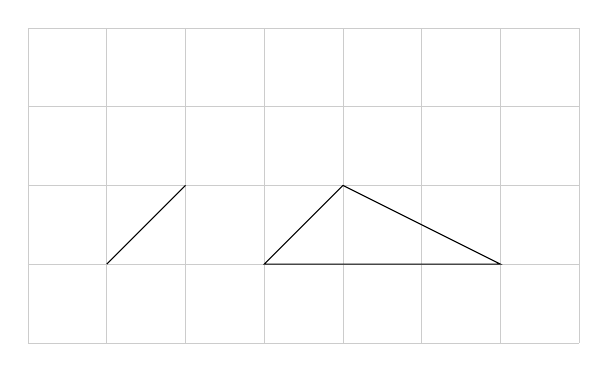
\begin{tikzpicture}
			\draw	[step=1cm,black,very thin, gray!40]  
					(-1.0,-1.0) grid (6,3);
			\draw	(0,0) -- (1,1)
					(2,0) -- (5,0) -- (3,1) -- cycle;
			\end{tikzpicture}

	%	------------------------------------------------ code	
		\begin{mdframed}[style=code_document, frametitle={code}]
			\begin{verbatim}
			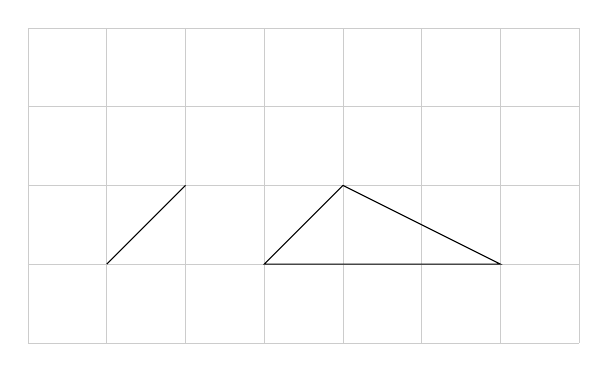
\begin{tikzpicture}
			\draw	[step=1cm,black,very thin, gray!40]  
					(-1.0,-1.0) grid (6,3);
			\draw	(0,0) -- (1,1)
					(2,0) -- (5,0) -- (3,1) -- cycle;
			\end{tikzpicture}
			\end{verbatim}
		\end{mdframed}



%	-----------------------------------------------------------  section
	\section{Horizontal and Vertical Connections}
	
		\paragraph{Horizontal and Vertical Connections}

			\tikz\draw	(0.0,0.0) -| (2.0,0.5)
						(1.0,1.0) -| (3.0,0.0);

	%	------------------------------------------------ code	
		\begin{mdframed}[style=code_document, frametitle={code}]
			\begin{verbatim}
			\tikz\draw	(0.0,0.0) -| (2.0,0.5)
						(1.0,1.0) -| (3.0,0.0);
			\end{verbatim}
		\end{mdframed}

		\paragraph{Horizontal and Vertical Connections}

			\tikz\draw	(0.0,0.0) |- (2.0,0.5)
						(1.0,1.0) |- (3.0,0.0);

	%	------------------------------------------------ code	
		\begin{mdframed}[style=code_document, frametitle={code}]
			\begin{verbatim}
			\tikz\draw	(0.0,0.0) -| (2.0,0.5)
						(1.0,1.0) -| (3.0,0.0);
			\end{verbatim}
		\end{mdframed}



%	-----------------------------------------------------------  section    relative and Incremental Coordinates
	\section{relative and Incremental Coordinates}


		\paragraph{relative and Incremental Coordinates}

		\tikzset{help lines/.style={ultra thin, blue!30}};
		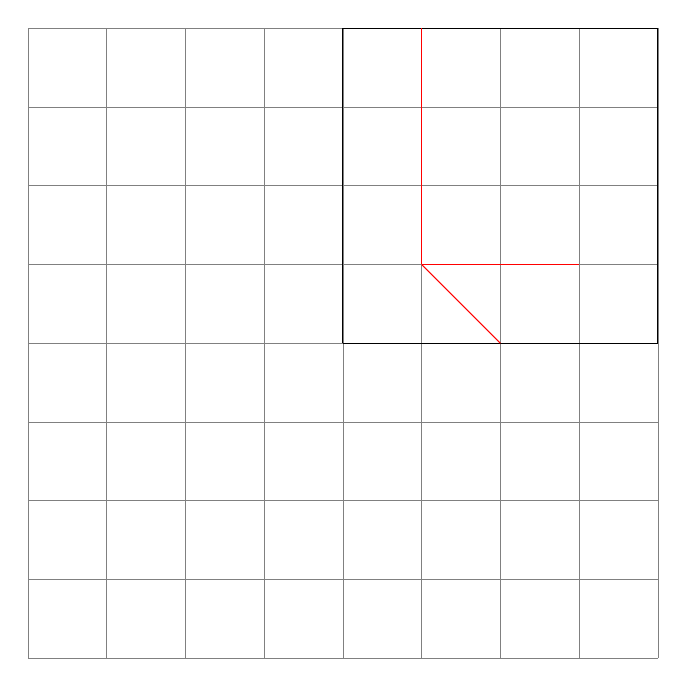
\begin{tikzpicture}
		\draw 	[help lines] (-4,-4) grid (4,4);
		\draw (0,0) -- (4,0) -- (4,4) -- (0,4) -- (0,0);
		\draw [red] (1,1) -- (+2,0);
		\draw [red] (1,1) -- +(2,0);
		\draw [red] (1,1) -- ++(0,3);
		\end{tikzpicture}
	

		\clearpage
		\paragraph{relative Coordinates : 첫번재 점을 원점으로 해서 }

			\tikzset{help lines/.style={ultra thin, blue!30}}
			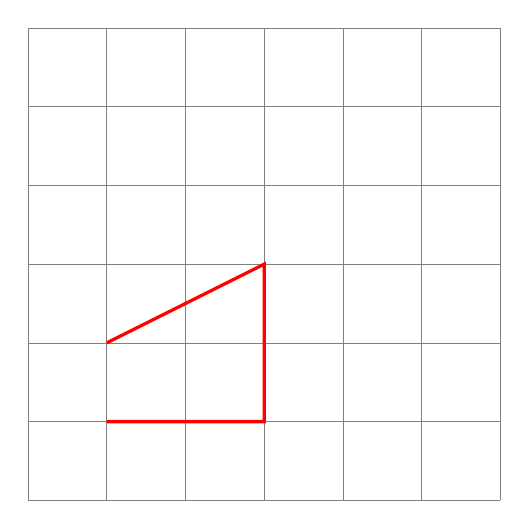
\begin{tikzpicture}
			\draw 	[help lines] (0,0) grid (6,6);
			\draw [red, very thick] 	(1,1) -- 
						+(2,0) --
						+(2,2) --
						+(0,1);
			\end{tikzpicture}

	%	------------------------------------------------ code	
		\begin{mdframed}[style=code_document, frametitle={code}]
			\begin{verbatim}
			\draw (1,1) -- +(2,0) -- +(2,2) -- +(0,1);
			\end{verbatim}
		\end{mdframed}


		\paragraph{Incremental Coordinates : 누적 }

			\tikzset{help lines/.style={ultra thin, blue!30}};
			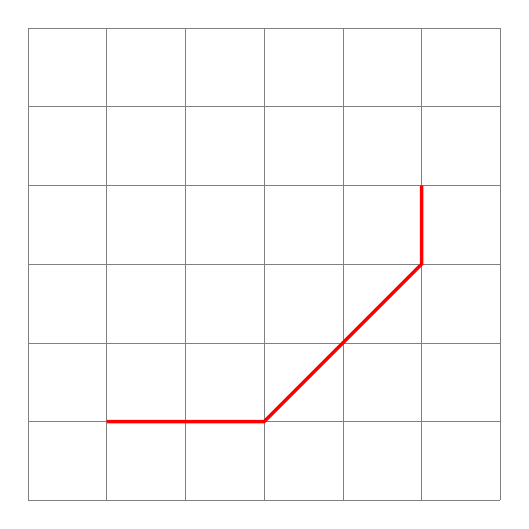
\begin{tikzpicture}
			\draw 	[help lines] (0,0) grid (6,6);
			\draw 	[red, very thick] (1,1) -- 
						++(2,0) --
						++(2,2) --
						++(0,1);
			\end{tikzpicture}




	%	------------------------------------------------ code	
		\begin{mdframed}[style=code_document, frametitle={code}]
			\begin{verbatim}
			\draw (1,1) -- ++(2,0) -- ++(2,2) -- ++(0,1);
			\end{verbatim}
		\end{mdframed}



	\clearpage
	\paragraph{fill}
		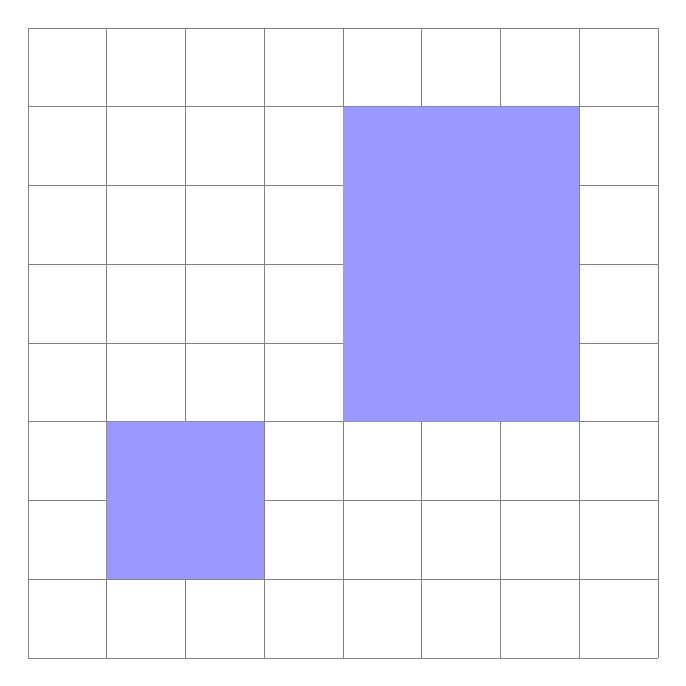
\begin{tikzpicture}
		\draw [help lines] (-3,-3) grid (5,5);
		\fill[blue!40!white] 	(-2,-2) rectangle (0,0) 
						+(1,0) rectangle +(4,4);
		\end{tikzpicture}


	%	------------------------------------------------ code	
		\begin{mdframed}[style=code_document, frametitle={code}]
		\begin{verbatim}
		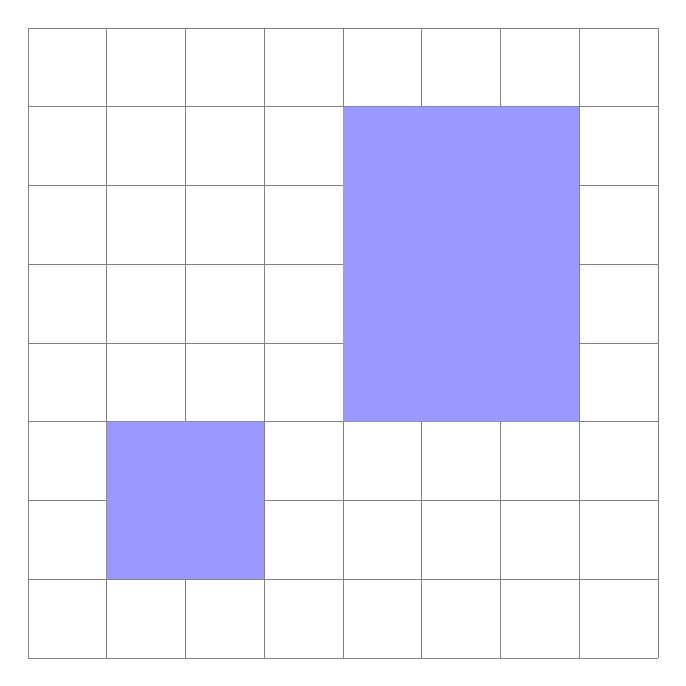
\begin{tikzpicture}
		\draw [help lines] (-3,-3) grid (5,5);
		\fill[blue!40!white] 	(-2,-2) rectangle (0,0) 
						+(1,0) rectangle +(4,4);
		\end{tikzpicture}
		\end{verbatim}
		\end{mdframed}


%	-----------------------------------------------------------  section    노드
	\section{node}



%	-----------------------------------------------------------  section    Labels
	\section{node Labels}



%	-----------------------------------------------------------  section    Shapes
	\section{node Shapes}



%	-----------------------------------------------------------  section    node Shapes split
	\section{node Shapes split}


%	-----------------------------------------------------------  section    노드
	\section{node Option}





%	-----------------------------------------------------------  section    노드
	\section{coordinate labels}




%	-----------------------------------------------------------  section
	\section{move-To}








%	-----------------------------------------------------------  section    라인
	\section{Line-To}

	
		\paragraph{Line}
			\begin{tikzpicture}
			\draw (0,0) -- (4,0);
			\end{tikzpicture}
		%	------------------------------------------------ code	
			\begin{mdframed}[style=code_document, frametitle={code}]
			\begin{verbatim}
			\begin{tikzpicture}
			\draw (0,0) -- (4,0);
			\end{tikzpicture}
			\end{verbatim}
			\end{mdframed}
	
	
		\paragraph{Line}
			\begin{tikzpicture} [color=green]
			\draw				(0,2) -- (4,2);
			\draw	[color=red] 	(0,1) -- (4,1);
			\draw	[red] 												(0,0) -- (4,0);
			\end{tikzpicture}
	
		%	------------------------------------------------ code	
			\begin{mdframed}[style=code_document, frametitle={code}]
			\begin{verbatim}
			\begin{tikzpicture} [color=green]
			\draw				(0,2) -- (4,2);
			\draw	[color=red] 	(0,1) -- (4,1);
			\draw	[red] 		(0,0) -- (4,0);
			\end{tikzpicture}
			\end{verbatim}
			\end{mdframed}



%	-----------------------------------------------------------  section    라인
	\section{Line width}
	
	
		\paragraph{ultra thin} 	
			\tikz {\draw[ultra thin] (-1.5,0) -- (1.5,0) }
		%	------------------------------------------------ code	
			\begin{mdframed}[style=code_document, frametitle={code}]
			\begin{verbatim}
			\tikz {\draw[ultra thin] (-1.5,0) -- (1.5,0) }
			\end{verbatim}
			\end{mdframed}
		
		\paragraph{very thin} 	\tikz {\draw[very thin] (-1.5,0) -- (1.5,0) }
		\paragraph{thin} 		\tikz {\draw[thin] (-1.5,0) -- (1.5,0) }
		\paragraph{line} 		\tikz {\draw (-1.5,0) -- (1.5,0) }
		\paragraph{semithick} 	\tikz {\draw[semithick] (-1.5,0) -- (1.5,0) }
		\paragraph{thick} 		\tikz {\draw[thick] (-1.5,0) -- (1.5,0) }
		\paragraph{very thick}	\tikz {\draw[very thick] (-1.5,0) -- (1.5,0) }
		\paragraph{ultra thick}	\tikz {\draw[ultra thick] (-1.5,0) -- (1.5,0) }
		\paragraph{line width=1en}	\tikz {\draw[line width=1em] (-1.5,0) -- (1.5,0) }
	
	
%	-----------------------------------------------------------  section    점선 
	\section{Dashed and dotted Lines}




%	-----------------------------------------------------------  section    선과 화살표
	\section{Line and arrows}


	\paragraph{$<->$}	\tikz {\draw[very thick, <->] (-2.0,0) -- (2.0,0) }

	\paragraph{$|<->|$}	\tikz {\draw[very thick, |<->|] (-2.0,0) -- (2.0,0) }

	\paragraph{$->$}	\tikz {\draw[very thick, ->, >= angle 90] (-2.0,0) -- (2.0,0) }
	\paragraph{$->$}	\tikz {\draw[very thick, ->, >= angle 60] (-2.0,0) -- (2.0,0) }

	\paragraph{$->$}	\tikz {\draw[very thick, ->, >= triangle 90] (-2.0,0) -- (2.0,0) }
	\paragraph{$->$}	\tikz {\draw[very thick, ->, >= triangle 60] (-2.0,0) -- (2.0,0) }





%	-----------------------------------------------------------  section  
	\section{Box}

	\paragraph{square}
	
		\begin{tikzpicture}
		\draw (0,0) -- (4,0) -- (4,4) -- (0,4) -- (0,0);
		\end{tikzpicture}
		
	%	------------------------------------------------ code	
		\begin{mdframed}[style=code_document, frametitle={code}]
		\begin{verbatim}
		\begin{tikzpicture}
		\draw (0,0) -- (4,0) -- (4,4) -- (0,4) -- (0,0);
		\end{tikzpicture}
		\end{verbatim}
		\end{mdframed}

	
	
	
	\paragraph{square}
		\begin{tikzpicture}
		\draw (0,0) -- (4,0) -- (4,4) -- (0,4) -- cycle;
		\end{tikzpicture}
	%	------------------------------------------------ code	
		\begin{mdframed}[style=code_document, frametitle={code}]
		\begin{verbatim}
		\begin{tikzpicture}
		\draw (0,0) -- (4,0) -- (4,4) -- (0,4) -- cycle;
		\end{tikzpicture}
		\end{verbatim}
		\end{mdframed}

		
	
	\paragraph{square}
		\begin{tikzpicture}
		\draw (0,0) rectangle (4,4);
		\end{tikzpicture}

	%	------------------------------------------------ code	
		\begin{mdframed}[style=code_document, frametitle={code}]
		\begin{verbatim}
		\begin{tikzpicture}
		\draw (0,0) rectangle (4,4);
		\end{tikzpicture}
		\end{verbatim}
		\end{mdframed}
	%	------------------------------------------------ code	


	\paragraph{square}
		\begin{tikzpicture}
		\draw (0,0) 	rectangle (4,4)
					rectangle (5,5);
		\end{tikzpicture}

	%	------------------------------------------------ code	
		\begin{mdframed}[style=code_document, frametitle={code}]
		\begin{verbatim}
		\begin{tikzpicture}
		\draw (0,0) 	rectangle (4,4)
					rectangle (5,5);
		\end{tikzpicture}
		\end{verbatim}
		\end{mdframed}
	%	------------------------------------------------ code	


	

%	-----------------------------------------------------------  section  
	\section{circle}


	\paragraph{circle}

		\begin{tikzpicture}
		\draw (3,3) circle (2cm);
		\end{tikzpicture}

	%	------------------------------------------------ code	
		\begin{mdframed}[style=code_document, frametitle={code}]
		\begin{verbatim}
		\begin{tikzpicture}
		\draw (3,3) circle (2cm);
		\end{tikzpicture}
		\end{verbatim}
		\end{mdframed}


	\paragraph{circle 2em}	
		\tikz {\draw circle (2em) }
	%	------------------------------------------------ code	
		\begin{mdframed}[style=code_document, frametitle={code}]
		\begin{verbatim}
		\tikz {\draw circle (2em) }
		\end{verbatim}
		\end{mdframed}
	
	\paragraph{circle 2cm}	\tikz {\draw circle (2cm) }


	\paragraph{redthickdashed}
		\begin{tikzpicture}
		\draw[red,thick,dashed] (2,2) circle (3cm);
		\end{tikzpicture}



%	-----------------------------------------------------------  section  ellipse
	\section{ellipse}

	\paragraph{ellipse}
		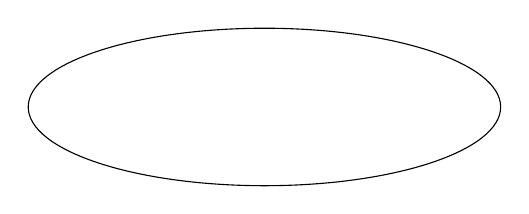
\begin{tikzpicture}
		\draw (2,2) ellipse (3cm and 1cm);
		\end{tikzpicture}
	%	------------------------------------------------ code	
		\begin{mdframed}[style=code_document, frametitle={code}]
		\begin{verbatim}
		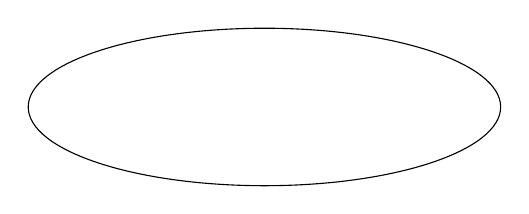
\begin{tikzpicture}
		\draw (2,2) ellipse (3cm and 1cm);
		\end{tikzpicture}
		\end{verbatim}
		\end{mdframed}

	\paragraph{ellipse}
		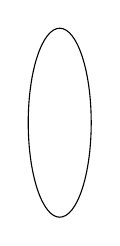
\begin{tikzpicture} [scale=0.4]
		\draw (2,2) ellipse (1cm and 3cm);
		\end{tikzpicture}
	%	------------------------------------------------ code	
		\begin{mdframed}[style=code_document, frametitle={code}]
		\begin{verbatim}
		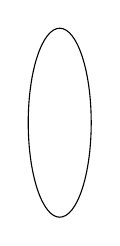
\begin{tikzpicture} [scale=0.4]
		\draw (2,2) ellipse (1cm and 3cm);
		\end{tikzpicture}
		\end{verbatim}
		\end{mdframed}


%	-----------------------------------------------------------  section  arc
	\section{arc}

	\paragraph{arc}
		\begin{tikzpicture}
		\draw	[help lines] (0,0) grid (4,4);
		\draw 	(0,0) arc (30:90:4cm);
		\draw 	(4,0) arc (30:90:4cm);
		\draw 	(4,0) arc (45:90:4cm);
		\draw 	(4,0) arc (90:180:3cm);
		\end{tikzpicture}

	%	------------------------------------------------ code	
		\begin{mdframed}[style=code_document, frametitle={code}]
		\begin{verbatim}
		\begin{tikzpicture}
		\draw	[help lines] (0,0) grid (4,4);
		\draw 	(0,0) arc (30:90:4cm);
		\draw 	(4,0) arc (30:90:4cm);
		\end{tikzpicture}
		\end{verbatim}
		\end{mdframed}


		


%	-----------------------------------------------------------  section  parabola
	\section{parabola}

	\paragraph{parabola}
	
		\begin{tikzpicture}
		\draw (0,0) parabola (4,4);
		\end{tikzpicture}
	


%	-----------------------------------------------------------  section  
	\section{char}


		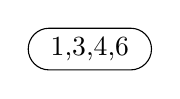
\begin{tikzpicture}[baseline=(char.base)]
		\node(char)[	draw,
					fill=white,  
					shape=rounded rectangle,
%					drop shadow={opacity=.5,shadow xshift=0pt},
					minimum width=1.8cm]
					{1,3,4,6};
		\end{tikzpicture}

	%	------------------------------------------------ code	
		\begin{mdframed}[style=code_document, frametitle={code}]
		\begin{verbatim}
		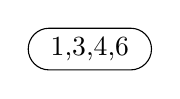
\begin{tikzpicture}[baseline=(char.base)]
		\node(char)[	draw,
					fill=white,  
					shape=rounded rectangle,
%					drop shadow={opacity=.5,shadow xshift=0pt},
					minimum width=1.8cm]
					{1,3,4,6};
		\end{tikzpicture}
		\end{verbatim}
		\end{mdframed}





		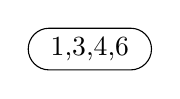
\begin{tikzpicture}
		\node(char)[	draw,
					fill=white,  
					shape=rounded rectangle,
%					drop shadow={opacity=.5,shadow xshift=0pt},
					minimum width=1.8cm]
					{1,3,4,6};
		\end{tikzpicture}


	%	------------------------------------------------ code	
		\begin{mdframed}[style=code_document, frametitle={code}]
		\begin{verbatim}
		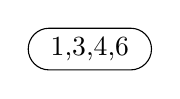
\begin{tikzpicture}
		\node(char)[	draw,
					fill=white,  
					shape=rounded rectangle,
%					drop shadow={opacity=.5,shadow xshift=0pt},
					minimum width=1.8cm]
					{1,3,4,6};
		\end{tikzpicture}
		\end{verbatim}
		\end{mdframed}


%	-----------------------------------------------------------  section  
	\section{원문자}

		\paragraph{node circle draw}		\hfill \\

		\tikz {\node [line width=1mm, circle, draw] at (0,0) {강도} }
		\tikz {\node [line width=1mm, circle, draw] at (0,0) {강도1111} }
		\tikz {\node [line width=1mm, circle, draw] at (0,0) {강도111111} }
		\tikz {\node [line width=1mm, circle, draw] at (0,0) {강도1111111} }
		\tikz {\node [line width=1mm, circle, draw] at (0,0) {강도11111111111} }
	

	%	------------------------------------------------ code	
		\begin{mdframed}[style=code_document, frametitle={code}]
		\begin{verbatim}
		\tikz {\node [line width=1mm, circle, draw] at (0,0) {강도} }
		\tikz {\node [line width=1mm, circle, draw] at (0,0) {강도1111} }
		\tikz {\node [line width=1mm, circle, draw] at (0,0) {강도111111} }
		\tikz {\node [line width=1mm, circle, draw] at (0,0) {강도1111111} }
		\tikz {\node [line width=1mm, circle, draw] at (0,0) {강도11111111111} }
		\end{verbatim}
		\end{mdframed}

		\paragraph{node circle=4em draw}		\hfill \\
		
		\begin{center}
		\tikz {\draw[line width=1mm, color=red] (0,0) circle (4em) node{test} }
		\tikz {\draw[line width=1mm, color=red] (0,0) circle (4em) node{test} }
		\tikz {\draw[line width=1mm, color=red] (0,0) circle (4em) node{\Large test} }
		\end{center}

	%	------------------------------------------------ code	
		\begin{mdframed}[style=code_document, frametitle={code}]
		\begin{verbatim}
		\tikz {\draw[line width=1mm, color=red] (0,0) circle (4em) node{test} }
		\tikz {\draw[line width=1mm, color=red] (0,0) circle (4em) node{test} }
		\tikz {\draw[line width=1mm, color=red] (0,0) circle (4em) node{\Large test} }
		\end{verbatim}
		\end{mdframed}

		\paragraph{node circle=4em draw 문자열의 길이가 긴 경우}		\hfill \\
	
		\tikz {\draw[line width=1mm, color=red] (0,0) circle (4em) node{test test} }
		\tikz {\draw[line width=1mm, color=red] (0,0) circle (4em) node{test test test} }
		\tikz {\draw[line width=1mm, color=red] (0,0) circle (4em) node{test test test test} }
		\tikz {\draw[line width=1mm, color=red] (0,0) circle (4em) node{test test test test test} }


	%	------------------------------------------------ code	
		\begin{mdframed}[style=code_document, frametitle={code}]
		\begin{verbatim}
		\tikz {\draw[line width=1mm, color=red] (0,0) circle (4em) node{test test} }
		\tikz {\draw[line width=1mm, color=red] (0,0) circle (4em) node{test test test} }
		\tikz {\draw[line width=1mm, color=red] (0,0) circle (4em) node{test test test test} }
		\tikz {\draw[line width=1mm, color=red] (0,0) circle (4em) node{test test test test test} }
		\end{verbatim}
		\end{mdframed}



%	------------------------------------------------------------------------------ 
	\section{원문자}

		\paragraph{text width = 4em}		\hfill \\
		
		\tikz {\draw[line width=0.4mm] (0,0) circle (4em) node[text width=4em]{test test} }
		\tikz {\draw[line width=0.4mm] (0,0) circle (4em) node{test test test} }
		\tikz {\draw[line width=0.4mm] (0,0) circle (4em) node{test test test test} }
		\tikz {\draw[line width=0.4mm] (0,0) circle (4em) node[text width=4em]{test test test test test} }

	%	------------------------------------------------ code	
		\begin{mdframed}[style=code_document, frametitle={code}]
		\begin{verbatim}
		\tikz {\draw[line width=0.4mm] (0,0) circle (4em) node[text width=4em]{test test} }
		\tikz {\draw[line width=0.4mm] (0,0) circle (4em) node{test test test} }
		\tikz {\draw[line width=0.4mm] (0,0) circle (4em) node{test test test test} }
		\tikz {\draw[line width=0.4mm] (0,0) circle (4em) node[text width=4em]{test test test test test} }
		\end{verbatim}
		\end{mdframed}

		\paragraph{text width = 6em}		\hfill \\
		
		\tikz {\draw[line width=0.4mm] (0,0) circle (4em) node[text width=6em]{test} }
		\tikz {\draw[line width=0.4mm] (0,0) circle (4em) node[text width=6em]{test test} }
		\tikz {\draw[line width=0.4mm] (0,0) circle (4em) node[text width=6em]{test test test} }
		\tikz {\draw[line width=0.4mm] (0,0) circle (4em) node[text width=6em]{test test test test test} }


	%	------------------------------------------------ code	
		\begin{mdframed}[style=code_document, frametitle={code}]
		\begin{verbatim}
		\tikz {\draw[line width=0.4mm] (0,0) circle (4em) node[text width=6em]{test} }
		\tikz {\draw[line width=0.4mm] (0,0) circle (4em) node[text width=6em]{test test} }
		\tikz {\draw[line width=0.4mm] (0,0) circle (4em) node[text width=6em]{test test test} }
		\tikz {\draw[line width=0.4mm] (0,0) circle (4em) node[text width=6em]{test test test test test} }
		\end{verbatim}
		\end{mdframed}

%	------------------------------------------------------------------------------ 
	\section{원문자}


		\paragraph{가운데 정렬, text width=6em}		\hfill \\
		
		\tikz {\draw[line width=0.4mm] circle (4em) node[align=center, text width=6em]{test test} }
		\tikz {\draw[line width=0.4mm] circle (4em) node[align=center, text width=6em]{test test test} }
		\tikz {\draw[line width=0.4mm] circle (4em) node[align=center, text width=6em]{test test test test} }
		\tikz {\draw[line width=0.4mm] circle (4em) node[align=center, text width=6em]{test test test test test} }


	%	------------------------------------------------ code	
		\begin{mdframed}[style=code_document, frametitle={code}]
		\begin{verbatim}
		\tikz {\draw[line width=0.4mm] circle (4em) node[align=center, text width=6em]{test test} }
		\tikz {\draw[line width=0.4mm] circle (4em) node[align=center, text width=6em]{test test test} }
		\tikz {\draw[line width=0.4mm] circle (4em) node[align=center, text width=6em]{test test test test} }
		\tikz {\draw[line width=0.4mm] circle (4em) node[align=center, text width=6em]{test test test test test} }
		\end{verbatim}
		\end{mdframed}

		
		\paragraph{가운데 정렬, text width=8em}		\hfill \\
		
		\tikz {\draw[line width=0.4mm] circle (4em) node[align=center, text width=8em]{test test} }
		\tikz {\draw[line width=0.4mm] circle (4em) node[align=center, text width=8em]{test test test} }
		\tikz {\draw[line width=0.4mm] circle (4em) node[align=center, text width=8em]{test test test test} }
		\tikz {\draw[line width=0.4mm] circle (4em) node[align=center, text width=8em]{test test test test test} }

	%	------------------------------------------------ code	
		\begin{mdframed}[style=code_document, frametitle={code}]
		\begin{verbatim}
		\tikz {\draw[line width=0.4mm] circle (4em) node[align=center, text width=8em]{test test} }
		\tikz {\draw[line width=0.4mm] circle (4em) node[align=center, text width=8em]{test test test} }
		\tikz {\draw[line width=0.4mm] circle (4em) node[align=center, text width=8em]{test test test test} }
		\tikz {\draw[line width=0.4mm] circle (4em) node[align=center, text width=8em]{test test test test test} }
		\end{verbatim}
		\end{mdframed}

		\paragraph{가운데 정렬, text width=8em}		\hfill \\
		
		\tikz {\draw[line width=0.4mm] circle (4em) node[align=center, text width=8em]{test \\ test test test test} }
		\tikz {\draw[line width=0.4mm] circle (4em) node[align=center, text width=8em]{test test \\  test test test} }
		\tikz {\draw[line width=0.4mm] circle (4em) node[align=center, text width=8em]{test test test \\ test test} }
		\tikz {\draw[line width=0.4mm] circle (4em) node[align=center, text width=8em]{test test test test \\ test} }

	%	------------------------------------------------ code	
		\begin{mdframed}[style=code_document, frametitle={code}]
		\begin{verbatim}
		\tikz {\draw[line width=0.4mm] circle (4em) node[align=center, text width=8em]{test \\ test test test test} }
		\tikz {\draw[line width=0.4mm] circle (4em) node[align=center, text width=8em]{test test \\  test test test} }
		\tikz {\draw[line width=0.4mm] circle (4em) node[align=center, text width=8em]{test test test \\ test test} }
		\tikz {\draw[line width=0.4mm] circle (4em) node[align=center, text width=8em]{test test test test \\ test} }
		\end{verbatim}
		\end{mdframed}



%	-----------------------------------------------------------  section  
	\section{사각 문자}

		\tikz {\draw[line width=1mm, color=gray] (0,0) rectangle node{1} (0.5,0.5) }
		\tikz {\draw[line width=1mm, color=gray] (0,0) rectangle node{1} (1,1) }
		\tikz {\draw[line width=1mm, color=gray] (0,0) rectangle node{1} (2,2) }
	
		\tikz {\draw[line width=1mm, color=gray] (0,0) rectangle node{1} (0.5,0.5) }
		누구나 건강한 삶을 누리도록
		
		\tikz {\draw[line width=1mm, color=gray] (0,0) rectangle node{1} (1,1) }
		누구나 건강한 삶을 누리도록
		
		\tikz {\draw[line width=1mm, color=gray] (0,0) rectangle node{1} (2,2) }
		누구나 건강한 삶을 누리도록

		\tikz {\draw[line width=1mm, color=gray] (0,0) rectangle node{Test} (2,2) }
		\tikz {\draw[line width=1mm, color=gray] (0,0) rectangle node{Test} (2,2) }
		\tikz {\draw[line width=1mm, color=gray] (0,0) rectangle node{Test} (2,2) }

		\paragraph{문자 위치 조정}		\hfill \\

		\tikz {\draw[line width=1mm, color=gray] rectangle node{Test} (2,2) }
		\tikz {\draw[line width=1mm, color=gray] rectangle node{Test} (2,2) }
		\tikz {\draw[line width=1mm, color=gray] rectangle node{Test} (2,2) }

		\tikz {\draw[line width=1mm, color=gray] rectangle (2,2) node{Test} }
		\tikz {\draw[line width=1mm, color=gray] rectangle (2,2) node{Test} }
		\tikz {\draw[line width=1mm, color=gray] rectangle (2,2) node{Test} }

		\tikz {\draw[line width=1mm, color=gray] node{Test} rectangle (2,2) }
		\tikz {\draw[line width=1mm, color=gray] node{Test} rectangle (2,2) }
		\tikz {\draw[line width=1mm, color=gray] node{Test} rectangle (2,2) }

		\paragraph{scale 적용}		\hfill \\

		\tikz {\draw[line width=1mm, color=gray, scale=2] (0,0) rectangle node{Test} (2,2) }
		\tikz {\draw[line width=1mm, color=gray, scale=2] (0,0) rectangle node{Test} (2,2) }
		\tikz {\draw[line width=1mm, color=gray, scale=2] (0,0) rectangle node{\large Test} (2,2) }
		

%	-----------------------------------------------------------  section  
	\section{사각 문자}

		\tikz {\draw[line width=0.4mm] rectangle node{Test} (2,2) }
		\tikz {\draw[line width=0.4mm] rectangle node{Test 내용 설명 } (12,2) }
		\\

		\tikz {\draw[line width=0.8mm] rectangle node{1} (2,2) }
		\tikz {\draw[line width=0.4mm] rectangle node{Test 내용 설명 } (12,2) }\\
		\tikz {\draw[line width=0.8mm] rectangle node{2} (2,2) }
		\tikz {\draw[line width=0.4mm] rectangle node{Test 내용 설명 } (12,2) } 
		\\


		\tikz {\draw[line width=0.8mm] rectangle node[text width=1em]{1} (2,2) }
		\tikz {\draw[line width=0.4mm] rectangle node[align=left, text width=20em]{Test 내용 설명 } (12,2) }\\
		\tikz {\draw[line width=0.8mm] rectangle node[text width=1em]{2} (2,2) }
		\tikz {\draw[line width=0.4mm] rectangle node[align=left, text width=20em]{Test 내용 설명 } (12,2) }



%	-----------------------------------------------------------  section  
	\section{mark}


		\begin{tikzpicture}
		\draw (0,0)--(10,0);
		\filldraw (0,0) circle (3pt);
		\filldraw ([xshift=-2pt,yshift=-2pt]10,0) rectangle ++(4pt,4pt);
		\node[fill=black,regular polygon, regular polygon sides=3,inner sep=1.5pt] at (5cm,0) {};
		
		\draw (0,-1)--(10,-1);
		\node at (0,-1) {\pgfuseplotmark{*}};
		\node at (5cm,-1) {\pgfuseplotmark{triangle*}};
		\node at (10cm,-1) {\pgfuseplotmark{square*}};
		
		\draw[mark=*] plot coordinates {(0,-2)} -- plot[mark=triangle*] coordinates {(5cm,-2)} --
		  plot[mark=square*] coordinates {(10cm,-2)};
		\end{tikzpicture}

%	-----------------------------------------------------------  section  
	\section{curve}


	\paragraph{curve}

		\begin{tikzpicture}
		\draw (0,0) .. controls (0,4) and (4,0) .. (4,4);
		\end{tikzpicture}
	%	------------------------------------------------ code	
		\begin{mdframed}[style=code_document, frametitle={code}]
		\begin{verbatim}
		\begin{tikzpicture}
		\draw (0,0) .. controls (0,4) and (4,0) .. (4,4);
		\end{tikzpicture}
		\end{verbatim}
		\end{mdframed}



%	-----------------------------------------------------------  section  
	\section{Filling}

	\paragraph{fill}
		
\begin{tikzpicture}
		\fill[blue!40!white] (0,0) rectangle (4,4);
		\fill[blue!40!red] (5,0) rectangle (9,4);
		\end{tikzpicture}


	%	------------------------------------------------ code	
		\begin{mdframed}[style=code_document, frametitle={code}]
		\begin{verbatim}
		
\begin{tikzpicture}
		\fill[blue!40!white] (0,0) rectangle (4,4);
		\fill[blue!40!red] (5,0) rectangle (9,4);
		\end{tikzpicture}
		\end{verbatim}
		\end{mdframed}




	\paragraph{filldraw}
		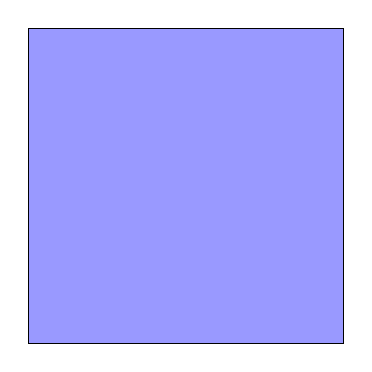
\begin{tikzpicture}
		\filldraw[fill=blue!40!white, draw=black] (0,0) rectangle (4,4);
		\end{tikzpicture}
	%	------------------------------------------------ code	
		\begin{mdframed}[style=code_document, frametitle={code}]
		\begin{verbatim}
		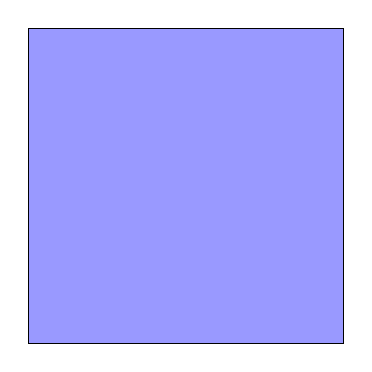
\begin{tikzpicture}
		\filldraw[fill=blue!40!white, draw=black] (0,0) rectangle (4,4);
		\end{tikzpicture}
		\end{verbatim}
		\end{mdframed}

	\paragraph{filldraw}
		
\begin{tikzpicture}
		\filldraw[fill=gray, draw=black] (0,0) rectangle (4,4);
		\end{tikzpicture}
	%	------------------------------------------------ code	
		\begin{mdframed}[style=code_document, frametitle={code}]
		\begin{verbatim}
		
\begin{tikzpicture}
		\filldraw[fill=gray, draw=black] (0,0) rectangle (4,4);
		\end{tikzpicture}
		\end{verbatim}
		\end{mdframed}

%	-----------------------------------------------------------  section  
	\section{Shading}

	\paragraph{shade1}

		
\begin{tikzpicture}
		\shade[left color=blue,right color=red] (0,0) rectangle (4,4);
		\end{tikzpicture}
		Instead of doing it from left to right we could do it from top to bottom.

	%	------------------------------------------------ code	
		\begin{mdframed}[style=code_document, frametitle={code}]
		\begin{verbatim}
		
\begin{tikzpicture}
		\shade	[left color=blue,right color=red] 
				(0,0) rectangle (4,4);
		\end{tikzpicture}
		\end{verbatim}
		\end{mdframed}

	\paragraph{shade 2}
		\begin{tikzpicture}
		\shade[top color=blue,bottom color=red] (0,0) rectangle (4,4);
		\end{tikzpicture}
		Or we could even change it by specifying an inner and outer colour like this.

	%	------------------------------------------------ code	
		\begin{mdframed}[style=code_document, frametitle={code}]
		\begin{verbatim}
		\begin{tikzpicture}
		\shade	[top color=blue,bottom color=red] 
				(0,0) rectangle (4,4);
		\end{tikzpicture}
		\end{verbatim}
		\end{mdframed}


	\paragraph{shade 3}
		\begin{tikzpicture}
		\shade[inner color=blue,outer color=red] (0,0) rectangle (4,4);
		\end{tikzpicture}
	%	------------------------------------------------ code	
		\begin{mdframed}[style=code_document, frametitle={code}]
		\begin{verbatim}
		\begin{tikzpicture}
		\shade	[inner color=blue,outer color=red] 
				(0,0) rectangle (4,4);
		\end{tikzpicture}
		\end{verbatim}
		\end{mdframed}


	\paragraph{shadedraw}

		\begin{tikzpicture}
		\shadedraw[inner color=blue,outer color=red, draw=black] (0,0) rectangle (4,4);
		\end{tikzpicture}

	%	------------------------------------------------ code	
		\begin{mdframed}[style=code_document, frametitle={code}]
		\begin{verbatim}
		\begin{tikzpicture}
		\shadedraw	[inner color=blue,outer color=red, draw=black] 
					(0,0) rectangle (4,4);
		\end{tikzpicture}
		\end{verbatim}
		\end{mdframed}

%	-----------------------------------------------------------  section  
	\section{Axes}

	\paragraph{Axes}

		\begin{tikzpicture}
		\draw[thick,->] (0,0) -- (5.5,0);
		\draw[thick,->] (0,0) -- (0,4.5);
		\end{tikzpicture}


	%	------------------------------------------------ code	
		\begin{mdframed}[style=code_document, frametitle={code}]
		\begin{verbatim}
		\begin{tikzpicture}
		\draw[thick,->] (0,0) -- (5.5,0);
		\draw[thick,->] (0,0) -- (0,4.5);
		\end{tikzpicture}
		\end{verbatim}
		\end{mdframed}


	\paragraph{plainarrows}

		\begin{tikzpicture}
		\draw[thick,->] (0,0) -- (4.5,0) node[anchor=north west] {x axis};
		\draw[thick,->] (0,0) -- (0,4.5) node[anchor=south east] {y axis};
		\end{tikzpicture}

	%	------------------------------------------------ code	
		\begin{mdframed}[style=code_document, frametitle={code}]
		\begin{verbatim}
		\begin{tikzpicture}
		\draw[thick,->] (0,0) -- (4.5,0) node[anchor=north west] {x axis};
		\draw[thick,->] (0,0) -- (0,4.5) node[anchor=south east] {y axis};
		\end{tikzpicture}
		\end{verbatim}
		\end{mdframed}


	\paragraph{foreach}

		\begin{tikzpicture}
		\foreach \x in {0,1,2,3,4}
		    \draw (\x cm,1pt) -- (\x cm,-1pt) node[anchor=north] {$\x$};
		\foreach \y in {0,1,2,3,4}
		    \draw (1pt,\y cm) -- (-1pt,\y cm) node[anchor=east] {$\y$};
		\end{tikzpicture}


	%	------------------------------------------------ code	
		\begin{mdframed}[style=code_document, frametitle={code}]
		\begin{verbatim}
		\begin{tikzpicture}
		\foreach \x in {0,1,2,3,4}
		    \draw (\x cm,1pt) -- (\x cm,-1pt) node[anchor=north] {$\x$};
		\foreach \y in {0,1,2,3,4}
		    \draw (1pt,\y cm) -- (-1pt,\y cm) node[anchor=east] {$\y$};
		\end{tikzpicture}
		\end{verbatim}
		\end{mdframed}


%	-----------------------------------------------------------  section    축 과 마크
	\section{axes with tick marks}


		\paragraph{axes} 	\hfill \\

							\tikz	{	\draw[->] (0,-4) -- (0,4) ;
								\draw[->] (-4,0) -- (4,0) ;
								\foreach \x in {-3, -2, -1, 1, 2, 3} \draw(\x, 2pt) -- (\x,-2pt);
								\foreach \y in {-3, -2, -1, 1, 2, 3} \draw(2pt,\y) -- (-2pt,\y);
							}




% 	==============================================================================  chapter  Flow chart
	\chapter{diagram}
	\minitoc				% Creating an actual minitoc


%	-----------------------------------------------------------  section  
	\section{circular diagram}

		\begin{center}
		\smartdiagramset{ 	border color=black				,%
%							back arrow disabled=true			,%
							module minimum width=6em 	,%
							module minimum height=3em 	,%
							uniform color list=gray!4 for 10 items				,%
							uniform arrow color=true			,%
							arrow color=black				,%
							}
		\smartdiagram[circular diagram]{단계 1, 단계 2, 단계 3, 단계 4}
		\end{center}

		\begin{center}
		\smartdiagram[circular diagram]{단계 1, 단계 2, 단계 3, 단계 4}
		\end{center}

		\smartdiagramset{ 	border color=black				,%
%							back arrow disabled=true			,%
							uniform color list=gray!4 for 10 items				,%
							module minimum width=6em 	,%
							module minimum height=3em 	,%
							uniform arrow color=true			,%
							arrow color=black				,%
							}
		\begin{center}
		\smartdiagram[circular diagram]{단계 1, 단계 2, 단계 3}
		\end{center}

		\begin{center}
		\smartdiagram[circular diagram]{단계 1, 단계 2}
		\end{center}

		\begin{center}
		\smartdiagram[circular diagram]{단계 1}
		\end{center}

		\begin{center}
		\smartdiagram[circular diagram:clockwise]{단계 1, 단계 2, 단계 3, 단계 4}
		\end{center}


%	-----------------------------------------------------------  section  
	\section{flow diagram}

		\paragraph{flow diagram}


		\begin{center}
		\smartdiagram[flow diagram]{단계 1, 단계 2, 단계 3, 단계 4}
		\end{center}

		\begin{center}
		\smartdiagram[flow diagram:horizontal]{단계 1, 단계 2, 단계 3, 단계 4}
		\end{center}

		\smartdiagramset{ 	border color=black				,%
%							back arrow disabled=true			,%
							uniform color list=gray!4 for 10 items				,%
							descriptive items y sep=4em 		,%
							module minimum width=6em 	,%
							module minimum height=4em 	,%
							back arrow disabled		=true 	,%
							arrow line width=2pt 			,%
							module x sep=8em 				,%  
							}
		\begin{center}
		\smartdiagram[flow diagram:horizontal]{단계 1, 단계 2, 단계 3}
		\end{center}


%	-----------------------------------------------------------  section  
	\section{descriptive diagram}

	%	---------------------------------------------------------- 
		\paragraph{descriptive}

		\smartdiagramset{ 	border color=black				,%
%							back arrow disabled=true			,%
							uniform color list=gray!4 for 10 items				,%
							descriptive items y sep=4em 		,%
							module minimum width=6em 	,%
							module minimum height=3em 	,%
							module x sep=4em 				,%  
							}
		\begin{center}
		\smartdiagram[descriptive diagram]{
				{단계 1, {단계 1에 대한 설명 }}, 
				{단계 2, {단계 1에 대한 설명 }},
				{단계 3, {단계 1에 대한 설명 }}, 
				{단계 4, {단계 1에 대한 설명 }}}
		\end{center}

	\paragraph{descriptive : descriptive items y sep=5em}

		\smartdiagramset{ 	border color=black				,%
							uniform color list=gray!4 for 10 items				,%
							descriptive items y sep=5em 		,%
							module minimum width=6em 	,%
							module minimum height=3em 	,%
							}
		\begin{center}
		\smartdiagram[descriptive diagram]{
				{단계 1, {단계 1에 대한 설명 }}, 
				{단계 2, {단계 1에 대한 설명 }},
				{단계 3, {단계 1에 대한 설명 }}, 
				{단계 4, {단계 1에 대한 설명 }}}
		\end{center}

	\paragraph{descriptive : descriptive items y sep=5em}

		\smartdiagramset{ 	border color=black				,%
							uniform color list=gray!4 for 10 items				,%
							descriptive items y sep=5em 		,%
							module minimum width=6em 	,%
							module minimum height=3em 	,%
							}
		\begin{center}
		\smartdiagram[descriptive diagram]{
				{단계 1, {단계 1에 대한 설명 }}, 
				{단계 2, {단계 1에 대한 설명 }},
				{단계 3, {단계 1에 대한 설명 }}, 
				{단계 4, {단계 1에 대한 설명 }}}
		\end{center}


%	-----------------------------------------------------------  section  
	\section{bubble diagram}


		\paragraph{bubble}

				\begin{center}
				\smartdiagram[bubble diagram]{단계 1, 단계 2, 단계 3, 단계 4}
				\end{center}
		
				\begin{center}
				\smartdiagram[bubble diagram]{단계 1, 단계 2, 단계 3}
				\end{center}
		
				\begin{center}
				\smartdiagram[bubble diagram]{단계 1, 단계 2}
				\end{center}
		
				\begin{center}
				\smartdiagram[bubble diagram]{단계 1}
				\end{center}

%	-----------------------------------------------------------  section  
	\section{constellation diagram}

		\paragraph{constellation}
	
				\begin{center}
				\smartdiagram[constellation diagram]{단계 0, 단계 1, 단계 2, 단계 3, 단계 4, 단계 5, 단계 6}
				\end{center}
			
				\begin{center}
				\smartdiagram[constellation diagram]{단계 1, 단계 2, 단계 3, 단계 4}
				\end{center}


%	-----------------------------------------------------------  section  
	\section{sequence diagram}
	
		\paragraph{sequence}

				\begin{center}
				\smartdiagram[sequence diagram]{단계 1, 단계 2, 단계 3, 단계 4}
				\end{center}


% 	==============================================================================  chapter  Flow chart
	\chapter{flow Chart}
	\minitoc				% Creating an actual minitoc
	

%	-----------------------------------------------------------  section  
	\section{flowchart}


		\paragraph{Prcess}

		\paragraph{Decision}

		\paragraph{Predefined Proces}

		\paragraph{Storage}

		\paragraph{Teminal}


		\clearpage
	%	------------------------------------------------------------------------------  FlowChart
		\begin{tikzpicture}

		\def\smbwd{2cm}

		\node (start) 	at (0,0) 		[	draw, terminal,
										minimum width=\smbwd,
										minimum height=0.5cm] {START};

		\node (predproc1) 	at (0,-1.5) 		[	draw, predproc, 
										align=left,
										minimum width=\smbwd,
										minimum height=1.0cm] {GET\\ DATA};


		\node (dec1) 		at (0,-3.5) 		[	draw, decision, 
										minimum width=\smbwd,
										minimum height=1.0cm] {C$<$3};


		\node (stg1) 		at (0,-5.5) 		[	draw, storage, 
										minimum width=\smbwd,
										minimum height=1.0cm] {STORAGE};

		\node (pro1) 		at (3,-5.5) 		[	draw, process, 
										minimum width=\smbwd,
										minimum height=1.0cm] {PROCESS};
		
		\coordinate (point_1)	at (0,-6.75);

		\node (end) 		at (0,-7.75) 	[	draw, terminal, 
										minimum width=\smbwd,
										minimum height=0.5cm] {END};

		\draw[->] 	(start) -- (predproc1);
		\draw[->] 	(predproc1) -- (dec1);
		\draw[->] 	(dec1) -| node [above] {YES} (pro1);
		\draw[->] 	(dec1) -- (stg1);
		\draw[->] 	(pro1) |- (point_1);
		\draw[->] 	(stg1) -- (point_1) -- (end);


		\end{tikzpicture}



		\clearpage
	%	------------------------------------------------------------------------------  FlowChart    Keyword 표시
		\begin{tikzpicture}
		
			\def\flowW{6.0cm}		% 수평크기 
			\def\flowH{1.0cm}		% 수직크기 
	
%			\node (NO_01) 	at (0,0.0) 	[	draw, process, minimum width=\flowW, minimum height=\flowH] {표면 조정};
			\node (NO_02) 	at (0,-2.0) 	
			[draw, process, minimum width=\flowW, minimum height=\flowH] 	{표면 조정};
			\node (NO_03) 	at (0,-4.0) 	
			[draw, process, minimum width=\flowW, minimum height=\flowH] 	{표면 조정};
			\node (NO_04) 	at (0,-6.0) 	
			[draw, process, minimum width=\flowW, minimum height=\flowH] 	{표면 조정};
			\node (NO_05) 	at (0,-8.0) 	
			[draw, process, minimum width=\flowW, minimum height=\flowH] 	{표면 조정};
			\node (NO_06) 	at (0,-10.0)	
			[draw, process, minimum width=\flowW, minimum height=\flowH] 	{표면 조정};
			\node (NO_06) 	at (0,-12.0)	
			[draw, process ] 													{표면 조정};
%			\node (NO_06) 	at (0,-12.0)	[	draw, process, text width=4cm,  minimum height=\flowH] {표면 조정};

		\end{tikzpicture}




		\clearpage
		강판 접착 공법의 일반 시공 순서도 \\
	%	------------------------------------------------------------------------------  FlowChart
		\begin{tikzpicture}
		
			\def\smbwd{4cm}		% 수평크기 
	
			\node (NO_01) 		at (0,0) 		[	draw, process,
											minimum width=\smbwd,
											minimum height=1.0cm] {표면 조정};
	

			\node (NO_02) 		at (0,-2.0) 		[	draw, process,
											minimum width=\smbwd,
											minimum height=1.0cm] {앵커 정착};


			\node (NO_03) 		at (0,-4.0) 		[	draw, process,
											minimum width=\smbwd,
											minimum height=1.0cm] {강판 부착};


			\node (NO_04) 		at (0,-6.0) 		[	draw, process,
											minimum width=\smbwd,
											minimum height=1.0cm] {에폭시 주입};

			\node (NO_05) 		at (0,-8.0) 		[	draw, process,
											minimum width=\smbwd,
											minimum height=1.0cm] {앵커 볼트 절단};

			\node (NO_06) 		at (0,-10.0) 		[	draw, process,
											minimum width=\smbwd,
											minimum height=1.0cm] {마감도장};


			\node (NO_11) 		at (7,0.0) 		[	draw, process,
											minimum width=9.0cm,
											minimum height=1.0cm] {박리, 열화부 제거, 표면 그라인딩, 균열 보수};

			\node (NO_12) 		at (7,-2.0) 		[	draw, process,
											minimum width=9.0cm,
											minimum height=1.0cm] {};

			\node (NO_13) 		at (7,-4.0) 		[	draw, process,
											minimum width=9.0cm,
											minimum height=1.0cm] {앵커를 이용하여 강판을 고정};

			\node (NO_14) 		at (7,-6.0) 		[	draw, process,
											minimum width=9.0cm,
											minimum height=1.0cm] {에폭시계 수지를 균일하게 도포};


			\node (NO_15) 		at (7,-8.0) 		[	draw, process,
											minimum width=9.0cm,
											minimum height=1.0cm] {지지대 설치 및 앵커볼트 절단};

			\node (NO_16) 		at (7,-10.0) 		[	draw, process,
											minimum width=9.0cm,
											minimum height=1.0cm] {필요에 따라 도료를 도포};


			\draw[->] 	(NO_01) -- (NO_02);
			\draw[->] 	(NO_02) -- (NO_03);
			\draw[->] 	(NO_03) -- (NO_04);
			\draw[->] 	(NO_04) -- (NO_05);
			\draw[->] 	(NO_05) -- (NO_06);
	

			\draw[->] 	(NO_01) -- (NO_11);
			\draw[->] 	(NO_02) -- (NO_12);
			\draw[->] 	(NO_03) -- (NO_13);
			\draw[->] 	(NO_04) -- (NO_14);
			\draw[->] 	(NO_05) -- (NO_15);
			\draw[->] 	(NO_06) -- (NO_16);

		
		
		\end{tikzpicture}





% 	==============================================================================  chapter  Flow chart
	\addtocontents{toc}{\protect\newpage}
	\chapter{Mind Map}
	\clearpage
	\minitoc				% Creating an actual minitoc
	

%	-----------------------------------------------------------  section  
	\section{mind map : Package 설정}

%	-----------------------------------------------------------  source code
	\begin{verbatim}

		%	=======================================================================================
		% 	tikz package
		% 	
		% 	--------------------------------- 	
			\usepackage{tikz}%
			\usetikzlibrary{arrows,positioning,shapes}
			\usetikzlibrary{mindmap}			

	\end{verbatim}


%	-----------------------------------------------------------  section  
	\section{mind map : 기본 형태}


	\paragraph{기본} \hfill 
		\begin{tikzpicture}
		\node{ShareLaTeX Tutorial Videos}
			    child { node {Beginners Series}}
			    child { node {Thesis Series}}
			    child { node {Beamer Series}}
			    child { node {TikZ Series}};
		\end{tikzpicture}

	\paragraph{기본} \hfill 
		\begin{tikzpicture}
			\node{ShareLaTeX Tutorial Videos}
			   child { node {Beginners Series}
			        child { node {First Document}}
			        child { node {Sections and Paragraphs}}
			        child { node {Mathematics}}
			        child { node {Images}}
			        child { node {bibliography}}
			        child { node {Tables and Matrices}}
			        child { node {Longer Documents}}
			    }
			    child { node {Thesis Series}
			        child { node {Basic Structure}}
			        child { node {Page Layout}}
			        child { node {Figures, Subfigures and Tables}}
			        child { node {Biblatex}}
			        child { node {Title Page}}
			    }
			    child { node {Beamer Series}
			        child { node {Getting Started}}
			        child { node {Text, Pictures and Tables}}
			        child { node {Blocks, Code and Hyperlinks}}
			        child { node {Overlay Specifications}}
			        child { node {Themes and Handouts}}
			    }
			    child { node {TikZ Series}
			        child { node {Basic Drawing}}
			        child { node {Geogebra}}
			        child { node {Flow Charts}}
			        child { node {Circuit Diagrams}}
			        child { node {Mind Maps}}
			    };
		\end{tikzpicture}

	\paragraph{기본} \hfill 

		\tikz[	mindmap,
				concept color=red!50,
				concept/.append style={fill={none}} 
				]
					\node [concept] 	{Root concept}
					child[grow=right] 	{node[concept] {Child concept}};


	\clearpage
	\paragraph{기본} \hfill 

			\begin{tikzpicture}
						[	mindmap,
							concept color=red!50,
							concept/.append style={fill={none}} 
						]
			\draw	[help lines] (-4,-4) grid (+16,+8);
			\path 	(-2,+0) coordinate (c1)
				 	(-1,+3) coordinate (c2)
				 	(+0,-3) coordinate (c3)
				 	(+2,-1) coordinate (c4);
			\draw 	[dashed]
					(c1) -- (c2) -- (c3)  -- (c4);	 	

			\node [draw, shape=rectangle] 	{Root concept}
							child[grow=right] 	{node[draw, shape=rectangle] {Child concept}
									child[grow=right] 	{node[rectangle] {Child concept}} };


			\node [draw, shape=rectangle] 	{Root concept}
							child[grow=right] 	{node[draw, shape=rectangle] {Child concept}
									child[grow=right] 	{node[draw, shape=rectangle] {Child concept}} 
									child[grow=45,level distance=16.0em] 		{node[draw, shape=rectangle] {Child concept}} 	
									child[grow=90] 		{node[draw, shape=rectangle] {Child concept}} };	

			\node [concept] 	{Root concept}
						child[grow=right] 	{node[concept] {Child concept}};

			\end{tikzpicture}












%	-----------------------------------------------------------  section  
	\section{mind map : 기본 세팅}


		\begin{tikzpicture}[	%
						mindmap,
						line width=2pt, 
						minimum size=5cm,
						text width=4cm, 
						text=black,
						align=flush center, 
						every node/.style=concept,
						every node/.append style={scale=1.0},
						concept color=black!60,
						grow cyclic,
						concept/.append style={fill={none}},
						level 1/.append style={level distance=4.5cm,sibling angle=90,	fill={none}},
						level 2/.append style={level distance=3.0cm,sibling angle=90,	fill={none}}
					]
				  \node [root concept] {Computational Complexity} % root
						[clockwise from=00]
						child 	[concept color=green!50!black]	{ node {Computational Problems}
							child { node {Problem Measures} } 
							child { node {Problem Aspects} }
					}
						child 		{ node {Computational Models}
							child { node {Turing Machines} }
							child { node {Random-Access Machines} }
					};
		\end{tikzpicture}

		\paragraph{mindmap style}

			\begin{verbatim}
			every mindmap
			\end{verbatim}

		\paragraph{node style}

			\begin{verbatim}
			every node/.style=concept,
			\end{verbatim}

		\paragraph{concept size}

			\begin{verbatim}
			every  minimum size=0.5cm
			\end{verbatim}

		\paragraph{concept line width}

			\begin{verbatim}
			line width=2pt, 
			\end{verbatim}

		\paragraph{concept color}

			\begin{verbatim}
			concept color=<color>
			every concept/.append style={fill={none}},
			\end{verbatim}


		\paragraph{concept text size}

			\begin{verbatim}
			text width=4cm, 
			\end{verbatim}

		\paragraph{concept text color}

			\begin{verbatim}
			text=black,
			\end{verbatim}

		\paragraph{append style - scale}

			\begin{verbatim}
			every node/.append style={scale=1.0},
			\end{verbatim}

		\paragraph{append style - fill}

			\begin{verbatim}
			every concept/.append style={fill={none}},
			\end{verbatim}

		\paragraph{growl}
			\begin{verbatim}
			grow cyclic,
			\end{verbatim}

		\paragraph{level}
			\begin{verbatim}
			level 1/.append style={level distance=4.5cm,sibling angle=45 },
			level 2/.append style={level distance=3.0cm,sibling angle=90 }
			\end{verbatim}



%	-----------------------------------------------------------  section  
	\section{mind map : map style 맵의 종류} 


		\paragraph{style}
			\begin{itemize}
			\item 	every mindmap
			\item 	small mindmap
			\item 	mindmap
			\item 	large mindmap
			\item 	huge mindmap
			\end{itemize}


		\paragraph{every mindmap style} \hfill \\
		concept의 크기와 거리를 넣어주어야 한다. \\
		\tikz		[every mindmap,
				concept color=red!50,
				minimum size=2cm,
				level distance=3cm]
					\node [concept] 	{Root}
					child[grow=right] 	{node[concept] {Child}};


		\paragraph{every mindmap style} \hfill \\
		\tikz		[	every mindmap,
					concept color=red!50]
					\node [concept] 	{Root concept}
					child[grow=right] 	{node[concept] {Child concept}};

		\clearpage
		\paragraph{small mindmap style} \hfill \\
		\tikz		[small mindmap,
				concept color=red!50,
				]
					\node [concept] 	{Root}
					child[grow=right] 	{node[concept] {Child}};

		\paragraph{mindmap style} \hfill \\
		\tikz[mindmap,concept color=red!50]
					\node [concept] 	{Root concept}
					child[grow=right] 	{node[concept] {Child concept}};

		\paragraph{large mindmap style} \hfill \\
		\tikz[large mindmap,concept color=red!50]
					\node [concept] 	{Root concept}
					child[grow=right] 	{node[concept] {Child concept}};

		\paragraph{huge mindmap style} \hfill \\
		\tikz[huge mindmap,concept color=red!50]
					\node [concept] 	{Root concept}
					child[grow=right] 	{node[concept] {Child concept}};



%	-----------------------------------------------------------  section  
	\section{mind map : 기본 단위 concept}


		\paragraph{concept} \hfill \\
		\tikz[mindmap,concept color=red!10] \node [concept] {강도};
		\tikz[mindmap,concept color=red!10] \node [concept] {내구성} ;
		\tikz[mindmap,concept color=black!10] \node [concept] {수밀성} ;
		\tikz[mindmap,concept color=black!10] \node [concept] {균열\\저항성} ;
		\tikz[mindmap,concept color=black!10] \node [concept] {강재\\보호} ;



		\paragraph{extra concept} \hfill \\
		\tikz[mindmap,concept color=red!10] \node [extra concept] {강도} ;
		\tikz[mindmap,concept color=red!10] \node [extra concept] {강도} ;
		\tikz[mindmap,concept color=red!10] \node [extra concept] {내구성} ;
		\tikz[mindmap,concept color=red!10] \node [extra concept] {수밀성} ;
		\tikz[mindmap,concept color=red!10] \node [extra concept] {균열\\저항성} ;
		\tikz[mindmap,concept color=red!10] \node [extra concept] {강재\\보호} ;

		\tikz[mindmap,concept color=black!10] \node [extra concept, concept color=red!10] {강도} ;


%	-----------------------------------------------------------  section  
	\section{mind map : annotation latex mindmap annotation position}


		\begin{tikzpicture}[	mindmap,
						minimum size=1.0cm,
						concept color=red!10,] 
						
			\node	[concept] (root) {강도};
			\node	[annotation,right] at (root.east) {\Large 1234567890} ;
		\end{tikzpicture}

		\begin{tikzpicture}[	mindmap,
						minimum size=1.0cm,
						concept color=red!10,
						every annotation={fill={red!20}} ] 
			\node	[concept] (root) {강도};
			\node	[annotation] at (root.east) {\Large 1234567890} ;
		\end{tikzpicture}

		\begin{tikzpicture}[	every mindmap,
						minimum size=1.0cm,
						concept color=red!10,
						every annotation={fill={red!20}} ] 
			\node	[concept] (root) {강도};
			\node	[annotation,right] at (root.east) {\Large 1234567890} ;
		\end{tikzpicture}

		\begin{tikzpicture}[	every mindmap,
						minimum size=1.0cm,
						concept color=red!10,
						every annotation={fill={red!20}} ] 
			\node	[concept] (root) {강도};
			\node	[annotation,left] at (root.east) {\Large 1234567890} ;
		\end{tikzpicture}

%	-----------------------------------------------------------  section  
	\section{latex mindmap annotation position}

		\paragraph{annotation position - left} \hfill \\
		\begin{tikzpicture}[	every mindmap,
						minimum size=1.0cm,
						concept color=red!10,
						every annotation={fill={red!20}} ] 
			\node	[concept] (root) {강도};
			\node	[	annotation,
						minimum size=1.0cm,
						fill=black!20,
						left=10em,
						align=center,
						text width=6.0cm,
						rotate=00] at (root.center) {\Large 1234567890} ;
		\end{tikzpicture}

		\paragraph{annotation position - right} \hfill \\
		\begin{tikzpicture}[	every mindmap,
						minimum size=1.0cm,
						concept color=red!10,
						every annotation={fill={red!20}} ] 
			\node	[concept] (root) {강도};
			\node	[	annotation,
						minimum size=1.0cm,
						fill=black!20,
						right=10em,
						align=center,
						text width=6.0cm,
						rotate=00] at (root.center) {\Large 1234567890} ;
		\end{tikzpicture}

		\paragraph{annotation position - above} \hfill \\
		\begin{tikzpicture}[	every mindmap,
						minimum size=1.0cm,
						concept color=red!10,
						every annotation={fill={red!20}} ] 
			\node	[concept] (root) {강도};
			\node	[	annotation,
						minimum size=1.0cm,
						fill=black!20,
						above=2em,
						align=center,
						text width=6.0cm,
						rotate=00] at (root.center) {\Large 1234567890} ;
		\end{tikzpicture}

		\paragraph{annotation position - below} \hfill \\
		\begin{tikzpicture}[	every mindmap,
						minimum size=1.0cm,
						concept color=red!10,
						] 
			\node	[concept] (root) {강도};
			\node	[	annotation,
						minimum size=1.0cm,
						fill=black!10,
						align=center,
						text width=6.0cm,
						below=2em,
						rotate=00] at (root.center) {\Large 1234567890} ;
		\end{tikzpicture}



%	-----------------------------------------------------------  section  
	\section{mind map : color}

		\paragraph{color} \hfill  \\
		concept color=black!10 \\
		text=red \\

		\tikz[	mindmap, 
				concept color=black!10, 
				text=red
				]	%
				\node 	[concept] 						{\Large 강도} 
				child	[concept color=red!5, grow=00] {node[concept] {\Large 강도-1} } ;

		\paragraph{color} \hfill  \\
		concept color=black!80\\
		text=white\\

		\tikz[mindmap, concept color=black!80, text=white]	%
				\node [concept] {\Large 강도} 
				child[concept color=black!80, text=white,  grow=00] {node[concept] {강도-1} } ;




%	-----------------------------------------------------------  section  
	\section{mind map : size}

		\paragraph{concept size} \hfill \\
		\tikz[mindmap,minimum size=0.5cm, concept color=red!10] 		\node [concept] {강도} ;
		\tikz[mindmap,minimum size=1cm, concept color=red!10] 		\node [concept] {1cm} ;
		\tikz[mindmap,minimum size=2cm, concept color=red!10] 		\node [concept] {2cm} ;
		\tikz[mindmap,minimum size=3cm, concept color=black!10]		\node [concept] {3cm 수밀성} ;
		\tikz[mindmap,minimum size=4cm, concept color=black!10] 		\node [concept] {4cm 균열\\저항성} ;
		\tikz[mindmap,minimum size=5cm, concept color=black!10] 		\node [concept] {5cm 강재\\보호} ;
		\tikz[mindmap,minimum size=4cm, concept color=black!10] 		\node [concept] {\Large 균열\\저항성} ;

		\paragraph{every mindmap size} \hfill \\
		\tikz[every mindmap,minimum size=0.5cm, concept color=red!10] 	\node [concept] {0.5cm} ;
		\tikz[every mindmap,minimum size=1cm, concept color=red!10] 		\node [concept] {1cm} ;
		\tikz[every mindmap,minimum size=2cm, concept color=red!10] 		\node [concept] {2cm} ;
		\tikz[every mindmap,minimum size=3cm, concept color=black!10]		\node [concept] {수밀성} ;
		\tikz[every mindmap,minimum size=4cm, concept color=black!10]		\node [concept] {\Large 균열\\저항성} ;
		\tikz[every mindmap,minimum size=5cm, concept color=black!10]		\node [concept] {강재\\보호} ;


%	-----------------------------------------------------------  section  
	\section{mind map : trees}


		\paragraph{grow} \hfill  \\

		\tikz[	mindmap, 
				text width=4cm, 
				align=flush center, 
				concept color=black!10,
				text=black		]	%
				\node 		[concept] {강도}  
					child	[concept color=red!5, grow=00] 	{	node[concept] 	{강도-1} } ;

		\tikz	[		mindmap,
						text width=4cm, 
						align=flush center, 
						every node/.style=concept,
						every node/.append style={scale=1.0},
						concept color=black!60,
						grow cyclic,
						concept/.append style={fill={none}},
						level 1/.append style={level distance=4.5cm,sibling angle=90,	fill={none}},
						level 2/.append style={level distance=3.0cm,sibling angle=90,	fill={none}}
					]
			\node 	[concept] 		{강도}  
			child		[grow=right] 	{node[concept] {강도 내구성 수밀성}  
				child	[grow=right] 	{node[concept] {강도-1} } } ;


		\tikz	[		mindmap,
						align=flush center, 
						every node/.style=concept,
						concept color=black,
						grow cyclic,
						concept/.append style={fill={none}},
						level 1/.append style={level distance=4.5cm,sibling angle=45 },
						level 2/.append style={level distance=3.0cm,sibling angle=90 }
					]
			\node 	[concept] 		{강도}  
			[clockwise from=-45]
			child		{node[concept] {강도 }}  
			child		{node[concept] {내구성}} 
			child		{node[concept] {수밀성}}  ;



		\tikz[mindmap, concept color=black!10]	%
				\node [concept] {강도} 	child[concept color=red!5, grow=000] {node[concept] {강도-1} }
									child[concept color=red!5, grow=030] {node[concept] {강도-2} }
									child[concept color=red!5, grow=060] {node[concept] {강도-3} }
									child[concept color=red!5, grow=090] {node[concept] {강도-4} }
									child[concept color=red!5, grow=120] {node[concept] {강도-5} };





%	-----------------------------------------------------------  section  
	\section{mind map : clockwise }

		\tikz[	mindmap,
				line width=1pt, 
%				grow cyclic, 
				concept color=black!80,
				concept/.append style={fill={none}} 
				]
					\node [concept] 								{Root concept}
					child 		[grow=090,level distance=7cm]	{node[concept] 	{Child concept-1} 
						child	[grow=180,level distance=3cm]	{node[concept] 	{Child 180} }
						child	[grow=090,level distance=3cm]	{node[concept] 	{Child 090} }
					}
					child 		[grow=45]					{node[concept] 	{Child concept-2} 
						child	[grow=000,level distance=3cm]	{node[concept] 	{Child concept-2} }
						child	[grow=090,level distance=3cm]	{node[concept] 	{Child concept-3} }
					}
					child 		[grow=-060,sibling angle=90]{node[concept] 	{Child concept-3} 
							[clockwise from=60]
						child	[level distance=3cm]			{node[concept] 	{Child concept-2} }
						child	[level distance=4cm]			{node[concept] 	{Child concept-3} }
					}
					child 		[grow=-120]{node[concept] 	{Child concept-4} };



	\clearpage
	\begin{small}
	\begin{verbatim}

		\tikz[	mindmap,
				line width=1pt, 
%				grow cyclic, 
				concept color=black!80,
				concept/.append style={fill={none}} 
				]
					\node [concept] 								{Root concept}
					child 		[grow=090,level distance=7cm]	{node[concept] 	{Child concept-1} 
						child	[grow=180,level distance=3cm]	{node[concept] 	{Child 180} }
						child	[grow=090,level distance=3cm]	{node[concept] 	{Child 090} }
					}
					child 		[grow=45]					{node[concept] 	{Child concept-2} 
						child	[grow=000,level distance=3cm]	{node[concept] 	{Child concept-2} }
						child	[grow=090,level distance=3cm]	{node[concept] 	{Child concept-3} }
					}
					child 		[grow=-060,sibling angle=90]{node[concept] 	{Child concept-3} 
							[clockwise from=60]
						child	[level distance=3cm]			{node[concept] 	{Child concept-2} }
						child	[level distance=4cm]			{node[concept] 	{Child concept-3} }
					}
					child 		[grow=-120]{node[concept] 	{Child concept-4} };


	\end{verbatim}
	\end{small}

%	-----------------------------------------------------------  section  
	\section{mind map : clockwise }

		\tikz[	mindmap,
				line width=1pt, 					% 선 두께 지정
				concept color=black!80,			% 색깔 지정
				concept/.append style={fill={none}} 	% 채움 지정
				]
					\node [concept] 									{Root concept}
					[clockwise from=00]
					child 		[level distance=5cm]	{				node[concept] 	{Child concept-1} 
						child	[grow=090,level distance=3cm] {			node[concept] 	{Child 180} }
						child	[grow=000,level distance=3cm] {			node[concept] 	{Child 090} }
					}
					child 		[level distance=5cm,sibling angle=30] {	node[concept] 	{Child concept-2} 
							[clockwise from=00]
						child	[level distance=3cm,sibling angle=00]	{	node[concept] 	{Child concept-2} }
						child	[level distance=3cm,sibling angle=40]	{	node[concept] 	{Child concept-3} }
					}
					child 		[level distance=5cm,sibling angle=30] {	node[concept] 	{Child concept-3} 
							[clockwise from=-30]
						child	[level distance=3cm,sibling angle=00]	{	node[concept] 	{Child concept-2} }
						child	[level distance=3cm,sibling angle=40]	{	node[concept] 	{Child concept-3} }
					}
					child 		[level distance=5cm,sibling angle=30]	{	node[concept] 	{Child concept-4} 
							[clockwise from=-60]
						child	[level distance=3cm,sibling angle=00]	{	node[concept] 	{Child concept-2} }
						child	[level distance=3cm,sibling angle=40]	{	node[concept] 	{Child concept-3} }
					}
					child 		[level distance=5cm]				{	node[concept] 	{Child concept-5} }
					child 		[level distance=6cm]				{	node[concept] 	{Child concept-6} };



%	-----------------------------------------------------------  section  
	\section{mind map : clockwise  \& sibling angle }

		\paragraph{clockwise from = 90 sibling angle=30} \hfill  \\
		\tikz[	every mindmap,
				text width=4em, 
				align=flush center, 
				minimum size=1cm,
				concept color=black!80,
				concept/.append style={fill={none}} 
				]
					\node [concept] 				{Root concept}
					[clockwise from=90]
					child [sibling angle=30,level distance=3cm]	{	node[concept] 	{Child-1} 
							child 	{	node[concept] 	{1-1} }
							child {	node[concept] 	{1-2} } }
					child [sibling angle=30,level distance=3cm]	{	node[concept] 	{Child-2} }
					child [sibling angle=30,level distance=3cm]	{	node[concept] 	{Child-3} }
					child [sibling angle=30,level distance=3cm]	{	node[concept] 	{Child-4} };


		\paragraph{clockwise from = 90 sibling angle=-30} \hfill  \\
		\tikz[	every mindmap,
				text width=4em, 
				align=flush center, 
				minimum size=1cm,
				concept color=black!80,
				concept/.append style={fill={none}} 
				]
					\node [concept] 				{Root concept}
					[clockwise from=90]
					child [sibling angle=-30,level distance=3cm]	{	node[concept] 	{Child-1} 
							child 	{	node[concept] 	{1-1} }
							child {	node[concept] 	{1-2} } }
					child [sibling angle=-30,level distance=3cm]	{	node[concept] 	{Child-2} }
					child [sibling angle=-30,level distance=3cm]	{	node[concept] 	{Child-3} }
					child [sibling angle=-30,level distance=3cm]	{	node[concept] 	{Child-4} };



		\paragraph{clockwise from = 90 sibling angle=30, level distance=3cm} \hfill  \\
		\tikz[	every mindmap,
				text width=4em, 
				align=flush center, 
				minimum size=1cm,
				concept color=black!80,
				concept/.append style={fill={none}} 
				]
					\node [concept] 				{Root concept}
					[clockwise from=90,sibling angle=30,level distance=3cm]
					child 					{	node[concept] 	{Child-1} 
					[level distance=3cm]
							child 			{	node[concept] 	{1-1} }
							child 			{	node[concept] 	{1-2} } }
					child 					{	node[concept] 	{Child-2} }
					child 					{	node[concept] 	{Child-3} }
					child 					{	node[concept] 	{Child-4} };

		\paragraph{clockwise from = 90 sibling angle=30} \hfill  \\
		\tikz[	every mindmap,
				text width=4em, 
				align=flush center, 
				minimum size=1cm,
				concept color=black!80,
				concept/.append style={fill={none}} 
				]
					\node [concept] 				{Root concept}
					[clockwise from=90,sibling angle=30,level distance=5cm]
					child 					{	node[concept] 	{Child-1} 
					[level distance=3cm]
							child 			{	node[concept] 	{1-1} }
							child 			{	node[concept] 	{1-2} } }
					child 					{	node[concept] 	{Child-2} }
					child 					{	node[concept] 	{Child-3} }
					child 					{	node[concept] 	{Child-4} };



		\clearpage
		\paragraph{clockwise from = 0 sibling angle=30} \hfill  \\
		\tikz[	every mindmap,
				text width=4em, 
				align=flush center, 
				minimum size=1cm,
				concept color=black!80,
				concept/.append style={fill={none}} 
				]
					\node [concept] 				{Root concept}
					[clockwise from=0,sibling angle=30]
					child 					{	node[concept] 	{Child-1} 
					[level distance=3cm]
							child 			{	node[concept] 	{1-1} }
							child 			{	node[concept] 	{1-2} } }
					child [level distance=3cm]	{	node[concept] 	{Child-2} }
					child [level distance=3cm]	{	node[concept] 	{Child-3} }
					child [level distance=3cm]	{	node[concept] 	{Child-4} };

		\paragraph{clockwise from = 0,  sibling angle=30, level distance=3cm} \hfill  \\
		\tikz[	every mindmap,
				text width=4em, 
				align=flush center, 
				minimum size=1cm,
				concept color=black!80,
				concept/.append style={fill={none}} 
				]
					\node [concept] 						{Root concept}
					[clockwise from=0,sibling angle=30,level distance=3cm]
					child 					{	node[concept] 	{Child-1} 
					[level distance=3cm]
							child 			{	node[concept] 	{1-1} }
							child 			{	node[concept] 	{1-2} } }
					child 					{	node[concept] 	{Child-2} }
					child 					{	node[concept] 	{Child-3} }
					child 					{	node[concept] 	{Child-4} };

		\paragraph{clockwise from = 0,  sibling angle=30, level distance=5cm} \hfill  \\
		\tikz[	every mindmap,
				text width=4em, 
				align=flush center, 
				minimum size=1cm,
				concept color=black!80,
				concept/.append style={fill={none}} 
				]
					\node [concept] 					{Root concept}
					[clockwise from=0,sibling angle=30,level distance=5cm]
					child 					{	node[concept] 	{Child-1} 
					[level distance=3cm]
							child 			{	node[concept] 	{1-1} }
							child 			{	node[concept] 	{1-2} } }
					child 					{	node[concept] 	{Child-2} }
					child 					{	node[concept] 	{Child-3} }
					child 					{	node[concept] 	{Child-4} };


		\clearpage
		\paragraph{clockwise from = 00} \hfill  \\

		\tikz[	mindmap,
				grow cyclic, 
				concept color=black!80,
				concept/.append style={fill={none}} 
				]
					\node [concept] 				{Root concept}
					[clockwise from=00]
					child {			node[concept] 	{Child concept-1} 
							child {	node[concept] 	{Child concept-1-1} }
							child {	node[concept] 	{Child concept-1-2} }
						}
					child {			node[concept] 	{Child concept-2} }
					child {			node[concept] 	{Child concept-3} }
					child {			node[concept] 	{Child concept-4} };


%	-----------------------------------------------------------  section  
	\section{mind map}

		\begin{center}
		\tikz[	mindmap,
				line width=1pt, 
%				grow cyclic, 
				concept color=black!60,
				concept/.append style={fill={none}}
%				level 1/.style={level distance=4cm,sibling angle=90},
%				level 2/.style={level distance=4cm,sibling angle=45},
				]
					\node [concept] 		{갱외 \\선지보공}
%					[clockwise from=90]
				%	--------------------------------------------------------		
					child					[grow=-45,level distance=5cm] 	{node[concept] 	{부산방향} 
							child			[grow=240,level distance=3cm]	{node[concept]	{천공} 
									child	[grow=240,level distance=2cm] 	{node[concept] 	{9 M} }
									child	[grow=270,level distance=2cm] 	{node[concept] 	{6 M} }
									child	[grow=300,level distance=2cm] 	{node[concept] 	{차수} }
								}	
							child			[grow=-60,level distance=4cm]	{node[concept]	{그라우팅} 
									child	[grow=240,level distance=3cm] 	{node[concept] 	{보강} }
									child	[grow=300,level distance=3cm] 	{node[concept] 	{차수} }
								}	
						}
				%	--------------------------------------------------------		
					child					[grow=225,level distance=5cm] 	{node[concept] 	{울산방향} 
							child			[grow=240,level distance=3cm]	{node[concept]	{천공} 
									child	[grow=240,level distance=2cm] 	{node[concept] 	{9 M} }
									child	[grow=270,level distance=2cm] 	{node[concept] 	{6 M} }
									child	[grow=300,level distance=2cm] 	{node[concept] 	{차수} }
								}	
							child			[grow=-60,level distance=3cm]	{node[concept]	{그라우팅} 
									child	[grow=240,level distance=2cm] 	{node[concept] 	{보강} }
									child	[grow=300,level distance=2cm] 	{node[concept] 	{차수} }
								}	
						}
				%	--------------------------------------------------------		
					child					[grow=030,level distance=4cm] 	{	node[concept]	{자재} 
							child			[grow=000,level distance=3cm] 	{	node[concept] 	{시멘트} }
							child			[grow=030,level distance=3cm] 	{	node[concept] 	{혼화재} }
							child			[grow=060,level distance=3cm] 	{	node[concept] 	{철근} }
							child			[grow=090,level distance=3cm] 	{	node[concept] 	{그라우팅} }
						} ;
		\end{center}


%	-----------------------------------------------------------  section  
	\section{mind map : 	every mindmap	}

		\tikz[	every mindmap,
				minimum size=2cm,
				line width=1pt, 
				text width=4em, 
				align=flush center, 
%				grow cyclic, 
				concept color=black!80,
%				every concept/.append style={minimum size=4cm, text width=2cm}				
%				every concept/style={minimum size=4cm, text width=2cm}				
%				every concept/.style={minimum size=2cm},				
				concept/.append style={fill={none}} 
				]
					\node [concept] 								{Root}
					child 		[grow=090,level distance=4cm]	{node[concept] 	{concept-1} 
						child	[grow=180,level distance=4cm]	{node[concept] 	{180} }
						child	[grow=090,level distance=4cm]	{node[concept] 	{090} }
					}
					child 		[grow=045,level distance=4cm]	{node[concept] 	{concept-2} 
						child	[grow=000,level distance=4cm]	{node[concept] 	{Child concept-2} }
						child	[grow=090,level distance=4cm]	{node[concept] 	{Child concept-3} }
					}
					child 		[grow=-060,level distance=3cm]	{node[concept] 	{concept-3} 
							[clockwise from=00]
						child	[sibling angle=00,level distance=6cm]	{node[concept] 	{3-1} }
						child	[sibling angle=30,level distance=4cm]	{node[concept] 	{3-2} }
						child	[sibling angle=30,level distance=4cm]	{node[concept] 	{3-3} }
					}
					child		[grow=-180,level distance=3cm]	{node[concept] 	{concept-3} }
					child 		[grow=-120,level distance=4cm] 	{node[concept] 	{concept-4} };


%	-----------------------------------------------------------  section  
	\section{every concept\/.style=minimum size=3cm	}

		\tikz[	mindmap,
				line width=1pt, 
%				grow cyclic, 
				concept color=black!80,
%				every concept/.append style={minimum size=4cm, text width=2cm}				
%				every concept/style={minimum size=4cm, text width=2cm}				
				every concept/.style={minimum size=3cm},				
				concept/.append style={fill={none}} 
				]
					\node [concept] 											{Root concept}
					child 		[grow=090,level distance=8cm]	{node[concept] 	{Child concept-1} 
						child	[grow=180,level distance=4cm]	{node[concept] 	{Child 180} }
						child	[grow=090,level distance=4cm]	{node[concept] 	{Child 090} }
					}
					child 		[grow=45]					{node[concept] 	{Child concept-2} 
						child	[grow=000,level distance=4cm]	{node[concept] 	{Child concept-2} }
						child	[grow=090,level distance=4cm]	{node[concept] 	{Child concept-3} }
					}
					child 		[grow=-060,sibling angle=90]{node[concept] 	{Child concept-3} 
								[clockwise from=60]
						child	[sibling angle=00,level distance=4cm]	{node[concept] 	{Child 3-1} }
						child	[sibling angle=30,level distance=6cm]	{node[concept] 	{Child 3-2} }
					}
					child 		[grow=-120]{node[concept] 	{Child concept-4} };



%	-----------------------------------------------------------  section  
	\section{mind map}



		\begin{tikzpicture}[	mindmap,
					    every node/.style=concept,
					    concept color=black!20,
					    grow cyclic,
					    level 1/.append style={level distance=4.0cm,sibling angle=90},
					    level 2/.append style={level distance=4.5cm,sibling angle=45}
					    ]
		  \node [root concept] 
			{	최고의 가치 } % root
				%
			    	child [concept color=black!10] 	%
										{ node {일}
				child 						{ node {여기가 어디 1} } 
				child 						{ node {여기가 어디 2} }  }
				%
				child [concept color=blue!10] 	{ node {직장}
				child 						{ node {Turing Machines} }
				child 						{ node {Random-Access Machines} }
				child 						{ node {Random-Access Machines} }
				child 						{ node {Random-Access Machines} }  }
				%				
				child [concept color=blue!10] 	{ node {가정}
				child 						{ node {Turing Machines} }
				child 						{ node {Random-Access Machines} }
				child 						{ node {Random-Access Machines} }
				child 						{ node {Random-Access Machines} }  };
		\end{tikzpicture}




	\clearpage
%	-----------------------------------------------------------  source code
	\begin{verbatim}
		\begin{tikzpicture}[	mindmap,
					    every node/.style=concept,
					    concept color=black!20,
					    grow cyclic,
					    level 1/.append style={level distance=4.5cm,sibling angle=90},
					    level 2/.append style={level distance=4.5cm,sibling angle=45}
					    ]
		  \node [root concept] {	Computational Complexity} % root
						    	child [concept color=black!10] 	{ node {여기가 어디 0}
							child 						{ node {여기가 어디 1} } 
							child 						{ node {여기가 어디 2} }
						  }
							child [concept color=blue!10] 	{ node {Computational Models}
							child 						{ node {Turing Machines} }
							child 						{ node {Random-Access Machines} }
							child 						{ node {Random-Access Machines} }
							child 						{ node {Random-Access Machines} }
							child 						{ node {Random-Access Machines} }
						    };
		\end{tikzpicture}
	\end{verbatim}


%	-----------------------------------------------------------  section  
	\section{mind map : 사용예 - 원 하나}
	
		\paragraph{every mindmap은 줄바꿈이 안됨} \hfill \\
		\tikz	[every mindmap,minimum size=0.5cm, concept color=red!10] 		
				\node [concept] {4cm 균열\\저항성} ;
		\tikz	[every mindmap,minimum size=1cm, concept color=red!10] 		
				\node [concept] {4cm 균열\\저항성} ;
		\tikz	[every mindmap,minimum size=2cm, concept color=red!10] 		
				\node [concept] {4cm 균열\\저항성} ;
		\tikz	[every mindmap,minimum size=3cm, concept color=black!10]		
				\node [concept] {4cm 균열\\저항성} ;
		\tikz	[every mindmap,minimum size=4cm, concept color=black!10] 		
				\node [concept] {4cm 균열\\저항성} ;
		\tikz	[every mindmap,minimum size=5cm, concept color=black!10] 		
				\node [concept] {4cm 균열\\저항성} ;
				
		\paragraph{mindmap은 줄바꿈이 됨} \hfill \\
		\tikz	[mindmap,minimum size=0.5cm, concept color=red!10] 		
				\node [concept] {강도} ;
		\tikz	[mindmap,minimum size=1cm, concept color=red!10] 		
				\node [concept] {1cm} ;
		\tikz	[mindmap,minimum size=2cm, concept color=red!10] 		
				\node [concept] {2cm} ;
		\tikz	[mindmap,minimum size=3cm, concept color=black!10]		
				\node [concept] {3cm 수밀성} ;
		\tikz	[mindmap,minimum size=4cm, concept color=black!10] 		
				\node [concept] {4cm 균열\\저항성} ;
		\tikz	[mindmap,minimum size=5cm, concept color=black!10] 		
				\node [concept] {5cm 강재\\보호} ;
		\tikz	[mindmap,minimum size=4cm, concept color=black!10] 		
				\node [concept] {\Large 균열\\저항성} ;





		\clearpage
		\paragraph{원 1개} \hfill \\
		%	----------------------------------------------- mind map
		%	1개
		%	----------------------------------------------- mind map
			\begin{center}
			\tikz			[mindmap, text width=4em, concept/.append style={fill={none}}]
				\node 	[concept,minimum size=2cm, concept color=black!80]	{Root concept};
			\end{center}

		\paragraph{원 2개} \hfill \\
		%	----------------------------------------------- mind map
		%	2개
		%	----------------------------------------------- mind map
			\begin{center}
			\tikz			[mindmap, text width=4em, concept/.append style={fill={none}}]
				\node 	[concept,minimum size=2cm, concept color=black!80]	{Root concept};
			\hspace{4em}
			\tikz			[mindmap, text width=4em, concept/.append style={fill={none}}]
				\node 	[concept,minimum size=2cm, concept color=black!80]	{Root concept};
			\end{center}



		\paragraph{원 3개} \hfill \\
		%	----------------------------------------------- mind map
		%	3개
		%	----------------------------------------------- mind map
			\begin{center}
			\tikz			[mindmap, text width=4em, concept/.append style={fill={none}}]
				\node 	[concept,minimum size=2cm, concept color=black!80]	{Root concept};
			\hspace{1em}
			\tikz			[mindmap, text width=4em, concept/.append style={fill={none}}]
				\node 	[concept,minimum size=2cm, concept color=black!80]	{Root concept};
			\hspace{1em}
			\tikz			[mindmap, text width=4em, concept/.append style={fill={none}}]
				\node 	[concept,minimum size=2cm, concept color=black!80]	{Root concept};
			\end{center}

		\paragraph{원 4개} \hfill \\
		%	----------------------------------------------- mind map
		%	4개
		%	----------------------------------------------- mind map
			\begin{center}
			\tikz			[mindmap, text width=5em, concept/.append style={fill={none}}]
				\node 	[concept,minimum size=3cm, concept color=black!80]	{전위차\\작정법};
			\hspace{0em}
			\tikz			[mindmap, text width=5em, concept/.append style={fill={none}}]
				\node 	[concept,minimum size=3cm, concept color=black!80]	{흡광\\광도법};
			\hspace{0em}
			\tikz			[mindmap, text width=5em, concept/.append style={fill={none}}]
				\node 	[concept,minimum size=3cm, concept color=black!80]	{질산은\\적정법};
			\hspace{0em}
			\tikz			[mindmap, text width=5em, concept/.append style={fill={none}}]
				\node 	[concept,minimum size=3cm, concept color=black!80]	{간이\\염화물 측정기};
			\end{center}

%	-----------------------------------------------------------  section  
	\section{mind map : 사용예 - 원 둘}

		\paragraph{minimum size = 3cm} \hfill  \\
		%	----------------------------------------------- mind map
			\begin{center}
			\tikz[	mindmap,
					every node/.style=concept,
					text width=4em, 
					every concept/.style={minimum size=3cm},
					concept color=black!80,
					concept/.append style={fill={none}} 
					]
					\node 			 							{Root concept}
						child		[grow=0,level distance=6cm] 	{node	{Child concept}};
			\end{center}


		\paragraph{clockwise from = 0} \hfill  \\
		%	----------------------------------------------- mind map
			\begin{center}
			\tikz[	mindmap,
					every node/.style=concept,
					text width=4em, 
					line width=1.0mm,
					concept color=black!80,
					every concept/.style={minimum size=3cm},
					concept/.append style={fill={none}} ,
					level 1/.style={level distance=6cm},
					clockwise from=00,
					]
					\node 				{Root concept}
						child		{node	{Child concept}};
			\end{center}

		\paragraph{clockwise from = 30} \hfill  \\
		%	----------------------------------------------- mind map
			\begin{center}
			\tikz[	mindmap,
					every node/.style=concept,
					text width=4em, 
					concept color=black!80,
					every concept/.style={minimum size=3cm},
					concept/.append style={fill={none}} ,
					level 1/.style={level distance=6cm},
					clockwise from=30,
					]
					\node 				{Root concept}
						child		{node	{Child concept}};
			\end{center}

						
		\paragraph{clockwise from = 90} \hfill  \\
		%	----------------------------------------------- mind map
			\begin{center}
			\tikz[	mindmap,
					every node/.style=concept,
					text width=4em, 
					concept color=black!80,
					every concept/.style={minimum size=3cm},
					concept/.append style={fill={none}} ,
					level 1/.style={level distance=6cm},
					clockwise from=90,
					]
					\node 				{Root concept}
						child		{node	{Child concept}};
			\end{center}



		\clearpage
		\paragraph{수직 2단} \hfill  \\

		%	----------------------------------------------- mind map
		% 	수직 2단
		%	----------------------------------------------- mind map
			\begin{center}
			\tikz[	mindmap,
					every node/.style=concept,
					text width=8em, 
					line width=0.8mm,
					concept color=black!80,
					every concept/.style={minimum size=3cm},
					concept/.append style={fill={none}} ,
					level 1/.style={level distance=6cm},
					clockwise from=90,
					]
					\node 				{재료분리가\\일어날 경우}
						child		{node	{다짐수를\\줄인다}};
			\end{center}


		\clearpage
		\paragraph{수직 2단 4열 small mindmap } \hfill  \\
		%	----------------------------------------------- mind map
		% 	수직 3단 수령 2열
		%	----------------------------------------------- mind map
			\begin{center}
			\tikz[	small mindmap,
					every node/.style=concept,
					text width=6em, 
					line width=0.4mm,
					concept color=black!80,
					every concept/.style={minimum size=2cm},
					concept/.append style={fill={none}} ,
					level 1/.style={level distance=4cm},
					level 2/.style={level distance=4cm},
					clockwise from=-90,
					]
					\node 					{\normalsize 콘크리트\\내부의 온도}
							child		{node	{\normalsize 낮으면 증가			}};
			\hspace{0em}
			\tikz[	small mindmap,
					every node/.style=concept,
					text width=6em, 
					line width=0.4mm,
					concept color=black!80,
					every concept/.style={minimum size=2cm},
					concept/.append style={fill={none}} ,
					level 1/.style={level distance=4cm},
					level 2/.style={level distance=4cm},
					clockwise from=-90,
					]
					\node 					{\normalsize 콘크리트 \\표면의 함수상태}
							child		{node	{\normalsize 강도 저하		}};
			\hspace{0em}
			\tikz[	small mindmap,
					every node/.style=concept,
					text width=6em, 
					line width=0.4mm,
					concept color=black!80,
					every concept/.style={minimum size=2cm},
					concept/.append style={fill={none}} ,
					level 1/.style={level distance=4cm},
					level 2/.style={level distance=4cm},
					clockwise from=-90,
					]
					\node 					{\normalsize 탄산화}
							child		{node	{\normalsize 증가			}};
			\hspace{0em}
			\tikz[	small mindmap,
					every node/.style=concept,
					text width=6em, 
					line width=0.4mm,
					concept color=black!80,
					every concept/.style={minimum size=2cm},
					concept/.append style={fill={none}} ,
					level 1/.style={level distance=4cm},
					level 2/.style={level distance=4cm},
					clockwise from=-90,
					]
					\node 					{\normalsize 타격방향}
							child		{node	{\normalsize 수평방향}};
			\end{center}



		\clearpage
		\paragraph{수평 3단} \hfill  \\
		%	----------------------------------------------- mind map
		% 	수직 3단
		%	----------------------------------------------- mind map
			\begin{center}
			\tikz[	mindmap,
					every node/.style=concept,
					text width=8em, 
					line width=0.8mm,
					concept color=black!80,
					every concept/.style={minimum size=3cm},
					concept/.append style={fill={none}} ,
					level 1/.style={level distance=5cm},
					level 2/.style={level distance=5cm},
					clockwise from=00,
					]
					\node 					{재료분리가\\일어날 경우}
						child			{node	{다짐수를\\줄인다}
							child		{node	{다짐수를\\줄인다}}};

			\end{center}


		\clearpage
		\paragraph{수직 3단} \hfill  \\
		%	----------------------------------------------- mind map
		% 	수직 3단
		%	----------------------------------------------- mind map
			\begin{center}
			\tikz[	mindmap,
					every node/.style=concept,
					text width=8em, 
					line width=0.8mm,
					concept color=black!80,
					every concept/.style={minimum size=3cm},
					concept/.append style={fill={none}} ,
					level 1/.style={level distance=5cm},
					level 2/.style={level distance=5cm},
					clockwise from=-90,
					]
					\node 					{재료분리가\\일어날 경우}
						child			{node	{다짐수를\\줄인다}
							child		{node	{다짐수를\\줄인다}}};

			\end{center}


		\clearpage
		\paragraph{수직 3단 2열} \hfill  \\
		%	----------------------------------------------- mind map
		% 	수직 3단 2열
		%	----------------------------------------------- mind map
			\begin{center}
			\tikz[	mindmap,
					every node/.style=concept,
					text width=8em, 
					line width=0.8mm,
					concept color=black!80,
					every concept/.style={minimum size=3cm},
					concept/.append style={fill={none}} ,
					level 1/.style={level distance=5cm},
					level 2/.style={level distance=5cm},
					clockwise from=-90,
					]
					\node 					{재료분리가\\일어날 경우}
						child			{node	{다짐수를\\줄인다}
							child		{node	{다짐수를\\줄인다}}};
			\hspace{4em}
			\tikz[	mindmap,
					every node/.style=concept,
					text width=8em, 
					line width=0.8mm,
					concept color=black!80,
					every concept/.style={minimum size=3cm},
					concept/.append style={fill={none}} ,
					level 1/.style={level distance=5cm},
					level 2/.style={level distance=5cm},
					clockwise from=-90,
					]
					\node 					{재료분리가\\일어날 경우}
						child			{node	{다짐수를\\줄인다}
							child		{node	{다짐수를\\줄인다}}};


			\end{center}



		\clearpage
		\paragraph{수직 3단 2열 small mindmap } \hfill  \\
		%	----------------------------------------------- mind map
		% 	수직 3단 수령 2열
		%	----------------------------------------------- mind map
			\begin{center}
			\tikz[	small mindmap,
					every node/.style=concept,
					text width=6em, 
					line width=0.4mm,
					concept color=black!80,
					every concept/.style={minimum size=2cm},
					concept/.append style={fill={none}} ,
					level 1/.style={level distance=4cm},
					level 2/.style={level distance=4cm},
					clockwise from=-90,
					]
					\node 					{\normalsize 굳지 않은\\콘크리트}
						child			{node	{전 염화물\\이온량}
							child		{node	{0.3 kg}}};
			\hspace{4em}
			\tikz[	small mindmap,
					every node/.style=concept,
					text width=6em, 
					line width=0.4mm,
					concept color=black!80,
					every concept/.style={minimum size=2cm},
					concept/.append style={fill={none}} ,
					level 1/.style={level distance=4cm},
					level 2/.style={level distance=4cm},
					clockwise from=-90,
					]
					\node 					{\normalsize 굳은\\콘크리트}
						child			{node	{수용성\\염화물 이온량}
							child		{node	{시멘트 중량의 0.3\%}}};


			\end{center}


		%	----------------------------------------------- mind map
			\begin{center}
			\tikz[	mindmap,
					text width=4em, 
					every concept/.style={minimum size=3cm},
					concept color=red!50,
					concept/.append style={fill={none}} 
					]
					\node 	[concept] 										{Root concept}
					child	[grow=90,level distance=8cm] 	{node[concept] 	{Child concept}};
			\end{center}

		\clearpage
		\paragraph{3줄 } \hfill  \\
		%	----------------------------------------------- mind map
		% 	3줄
		%	----------------------------------------------- mind map
	
			\begin{center}
			\tikz[	mindmap,
					text width=6em, 
					minimum size=3cm,
					concept color=black!80,
					level 1/.style={level distance=5.0cm,sibling angle=30},
					concept/.append style={fill={none}} 
					]
					\node 	[concept] 				{50 mm}
							[clockwise from=15, every concept/.style={minimum size=2cm}]
					child	{	node[concept] 	{120 mm}}
					child	{	node[concept] 	{150 mm}} ;
			\end{center}
	
			\begin{center}
			\tikz[	mindmap,
					text width=6em, 
					minimum size=3cm,
					concept color=black!80,
					level 1/.style={level distance=5.0cm,sibling angle=00},
					concept/.append style={fill={none}} 
					]
					\node 	[concept] 				{80 mm}
							[clockwise from=00, every concept/.style={minimum size=2cm}]
					child	{	node[concept] 	{150 mm}} ;
			\end{center}
	
			\begin{center}
			\tikz[	mindmap,
					text width=6em, 
					minimum size=3cm,
					concept color=black!80,
					level 1/.style={level distance=5.0cm,sibling angle=00},
					concept/.append style={fill={none}} 
					]
					\node 	[concept] 				{60 mm}
							[clockwise from=00, every concept/.style={minimum size=2cm}]
					child	{	node[concept] 	{120 mm}} ;
			\end{center}	

		\clearpage

		\begin{center}
		\tikz		[mindmap, text width=6em,  every concept/.style={minimum size=4cm}, concept color=black!80, concept/.append style={fill={none}} ]
		\node 	[concept] {\large 슬러프 콘};
		\hspace{2em}
		\tikz		[mindmap, text width=6em,  every concept/.style={minimum size=4cm}, concept color=black!80, concept/.append style={fill={none}} ]
		\node 	[concept] {\large 다짐봉};
		\end{center}


		\begin{center}
		\tikz		[mindmap, text width=6em,  every concept/.style={minimum size=4cm}, concept color=black!80, concept/.append style={fill={none}} ]
		\node 	[concept] {\Large 슬러프 콘};
		\hspace{2em}
		\tikz		[mindmap, text width=6em,  every concept/.style={minimum size=4cm}, concept color=black!80, concept/.append style={fill={none}} ]
		\node 	[concept] {\Large 다짐봉};
		\end{center}


		%	----------------------------------------------- mind map
			\begin{center}
			\tikz		[mindmap, text width=4em,  every concept/.style={minimum size=4cm}, concept color=black!80, concept/.append style={fill={none}} ]
			\node 	[concept] {\Large 100};
			\hspace{1em}
			\tikz		[mindmap, text width=4em,  every concept/.style={minimum size=4cm}, concept color=black!80, concept/.append style={fill={none}} ]
			\node 	[concept] {\Large 200};
			\hspace{1em}
			\tikz		[mindmap, text width=4em,  every concept/.style={minimum size=4cm}, concept color=black!80, concept/.append style={fill={none}} ]
			\node 	[concept] {\Large 300};
			\end{center}

	
	
%	-----------------------------------------------------------  section  
	\section{mind map : 사용예 - 원 셋}
	
		\paragraph{상향 3개 } \hfill  \\
		%	----------------------------------------------- mind map
		% 	상향 3개
		%	----------------------------------------------- mind map
		\begin{center}
		\tikz[	mindmap,
				every node/.style=concept,
				text width=8em, 
				line width=0.4mm,
				concept color=black!80,
				every concept/.style={minimum size=3cm},
				concept/.append style={fill={none}},
				level 1/.style={level distance=5cm},
				level 2/.style={level distance=5cm},
				clockwise from=135,
				sibling angle=45,
				]
				\node 	[concept] 	{Root concept}
				child	{node[concept] 	{Child concept-1}}
				child	{node[concept] 	{Child concept-2}}
				child	{node[concept] 	{Child concept-3}} ;
		\end{center}

		\begin{center}
		\tikz[	mindmap,
				every node/.style=concept,
				text width=8em, 
				line width=0.4mm,
				concept color=black!80,
				every concept/.style={minimum size=3cm},
				concept/.append style={fill={none}},
				level 1/.style={level distance=5cm},
				level 2/.style={level distance=5cm},
				clockwise from=135,
				sibling angle=45,
				]
				\node 		{Root concept}
				child	{node	{Child concept-1}}
				child	{node	{Child concept-2}}
				child	{node	{Child concept-3}} ;
		\end{center}


		\paragraph{하향 3개 } \hfill  \\
		%	----------------------------------------------- mind map
		% 	하향 3개
		%	----------------------------------------------- mind map
		\begin{center}
		\tikz[	mindmap,
				every node/.style=concept,
				text width=8em, 
				line width=0.4mm,
				concept color=black!80,
				every concept/.style={minimum size=3cm},
				concept/.append style={fill={none}},
				level 1/.style={level distance=5cm},
				level 2/.style={level distance=5cm},
				clockwise from=-135,
				sibling angle=-45,
				]
				\node 	[concept] 	{Root concept}
				child	{node[concept] 	{Child concept-1}}
				child	{node[concept] 	{Child concept-2}}
				child	{node[concept] 	{Child concept-3}} ;
		\end{center}



		%	----------------------------------------------- mind map
		% 	하향 3개
		%	----------------------------------------------- mind map
		\begin{center}
		\tikz[	mindmap,
				text width=4em, 
				every concept/.style={minimum size=3cm},
				concept color=black!80,
				concept/.append style={fill={none}} 
				]
				\node 	[concept] 										{Root concept}
				child	[grow=-045,level distance=5cm] 	{node[concept] 	{Child concept}}
				child	[grow=-090,level distance=5cm] 	{node[concept] 	{Child concept}}
				child	[grow=-135,level distance=5cm] 	{node[concept] 	{Child concept}} ;
		\end{center}




%	-----------------------------------------------------------  section  
	\section{mind map : 사용예 - 원 다섯}
	

		\paragraph{하향 5개 } \hfill  \\
		%	----------------------------------------------- mind map
		% 	하향 5개
		%	----------------------------------------------- mind map
		\begin{center}
		\tikz[	mindmap,
				text width=4em, 
				every concept/.style={minimum size=2cm},
				concept color=red!50,
				concept/.append style={fill={none}} 
				]
				\node 	[concept] 										{Root concept}
				child	[grow=000,level distance=5cm] 	{node[concept] 	{Child 1}}
				child	[grow=-45,level distance=5cm] 	{node[concept] 	{Child 2}}
				child	[grow=-90,level distance=5cm] 	{node[concept] 	{Child 3}}
				child	[grow=-135,level distance=5cm] 	{node[concept] 	{Child 4}}
				child	[grow=180,level distance=5cm] 	{node[concept] 	{Child 5}} ;
		\end{center}


		\paragraph{하향 5개 } \hfill  \\
		%	----------------------------------------------- mind map
		% 	하향 5개
		%	----------------------------------------------- mind map
		\begin{center}
		\tikz[	mindmap,
				text width=4em, 
				concept color=black!50,
				concept/.append style={fill={none}} 
				]
				\node 	[concept] 										{Root concept}
				[every concept/.style={minimum size=2cm}]
				child	[grow=000,level distance=5cm] 	{node[concept] 	{Child 1}}
				child	[grow=-45,level distance=5cm] 	{node[concept] 	{Child 2}}
				child	[grow=-90,level distance=5cm] 	{node[concept] 	{Child 3}}
				child	[grow=-135,level distance=5cm] 	{node[concept] 	{Child 4}}
				child	[grow=180,level distance=5cm] 	{node[concept] 	{Child 5}} ;
		\end{center}


		\clearpage
		\paragraph{하향 5개 } \hfill  \\
		%	----------------------------------------------- mind map
		% 	하향 5개
		%	----------------------------------------------- mind map
		\begin{center}
		\tikz[	mindmap,
				text width=4em, 
				concept color=black!80,
				level 1/.style={level distance=5.5cm,sibling angle=45},
				concept/.append style={fill={none}} 
				]
				\node 	[concept] 				{Root concept}
						[clockwise from=00, every concept/.style={minimum size=2cm}]
				child	{	node[concept] 	{Child 1}}
				child	{	node[concept] 	{Child 2}}
				child	{	node[concept] 	{Child 3}}
				child	{	node[concept] 	{Child 4}}
				child	{	node[concept] 	{Child 5}} ;
		\end{center}


		\clearpage
		\paragraph{하향 5개 } \hfill  \\
		%	----------------------------------------------- mind map
		% 	하향 5개
		%	----------------------------------------------- mind map
		\begin{center}
		\tikz[	mindmap,
				text width=6em, 
				concept color=black!80,
				level 1/.style={level distance=5.5cm,sibling angle=45},
				concept/.append style={fill={none}} 
				]
				\node 	[concept] 				{워커빌리티\\시험}
						[clockwise from=00, every concept/.style={minimum size=3cm}]
				child	{	node[concept] 	{슬럼프}}
				child	{	node[concept] 	{구 관입}}
				child	{	node[concept] 	{비비 시험}}
				child	{	node[concept] 	{리몰딩 시험}}
				child	{	node[concept] 	{다짐계수 시험}} ;
		\end{center}

% 	==============================================================================  chapter  Flow chart
	\chapter{참고}
	\minitoc				% Creating an actual minitoc
	

%	-----------------------------------------------------------  section  
	\section{참고}


		부산시 연제구 교대로 13 지하  청출어람




% ------------------------------------------------------------------------------
% End document
% ------------------------------------------------------------------------------
\end{document}



% =================================================================================================== Part 혼화 재료

	%	------------------------------------------------------------------------------  table

			\begin{table} [h]
	
			\caption{잔 골재의 표준입도}  
			\label{tab:title} 
	
			\begin{center}
			\tabulinesep=0.4em
			\begin{tabu} to 0.8\linewidth { X[r] X[l] X[c]  }
			\tabucline [1pt,] {-}
			체의 호칭 치수 (mm)		& 체를 통화한 것의 질량 백분율(\%) \\
			\multicolumn{4}{c} {단위량} \\
			\tabucline [0.1pt,] {-}
			2.5	&100\\
			1.2	& 99 $\sim$ 100 \\
			0.6	& 60 $\sim$ 80 \\
			0.3	& 20 $\sim$ 50 \\
			0.15	&  5 $\sim$ 30 \\
			\tabucline [0.1pt,] {-}
			\end{tabu} 
			\end{center}
			\end{table}

%	------------------------------------------------------------------------------  문제

		\vfill
		\hrulefill
	
		\paragraph{문제}
		시멘트  제조 과정에서 시멘트의 응결을 지연시키는 역할을 하기 위하여 첨가하는 재료는 ?
			\begin{tabenum}[\bfseries(1)]%
			\item
			$ \text{석고}$
			\item
			$ \text{슬래그}$ \par
			\item
			$ \text{지연제}$
			\item
			$ \text{실리카} \rm (Si O_2 )$
			\end{tabenum}
		\paragraph{정답} 1
		\paragraph{풀이} 시멘트의 제조 과정에서 클링커에 응결 조절용으로 3$\sim$5\% 의 석고를 첨가, 분쇄하면 포틀랜드 시멘트가 얻어진다.



	%	------------------------------------------------------------------------------  문제

		\clearpage
		\vfill
		\hrulefill

		\begin{small}	
		\paragraph{문제}
		레미콘 공장 회수수 중 슬러지수를 혼합수로 사용하는 경우의 유의 사항에 관한 다음 설명 중 적당하지 않는 것은?

		\begin{tabbing}
		\=	① 슬러지 고형분은 시멘트 질량의 3\% 이하로 한다. \\
		\=	② 슬러지 고형분이 많은 경우에는 단위 수량을 증가시킨다. \\
		\=	③ 슬러지 고형분이 많은 경우에는 잔 골재율을 증가시킨다. \\
		\=	④ 슬러지 고형분이 많은 경우에는 AE제의 사용량을 증가 시킨다. 
		\end{tabbing}

		\paragraph{정답} ③
		\paragraph{풀이} 잔 골재율은 슬러지 고형분의 시멘트에 대한 첨가율 1\%에 대해 약 0.5\% 감소 시킨다.
		\end{small}	




	%	------------------------------------------------------------------------------  문제

		\clearpage
		\begin{small}	
		\begin{question}
		레디 믹스트 콘크리트에서 \textbf{회수수}를 혼합수로 사용할 경우 주의할 사항 중 틀린것은 ?
		\begin{enumerate}[label=\arabic*), topsep=0.0em, itemsep=-1.0em ]
			\item [①] 고강도 콘크리트의 경우 회수수를 사용하여서는 안된다. 
			\item [②] 슬러지수의 사용 시 \textbf{단위 슬러지 고형분}은 콘크리트 질량의 3\% 이하로 한다. 
			\item [③] 회수수의 품질 시험 항목은 4가지로 염소 이온량, 시멘트 응결 시간의 차, 모르타르 압축강도의 비, 단위 슬러지 고형분율 이다. 
			\item [④] 콘크리트를 배합할 때, 회수수 중에 함유된 슬러지 고형분은 물의 질량에는 포함되지 않는다. 
		\end{enumerate}
		\end{question}



		\begin{solution}
		해설
		\end{solution}
		\end{small}	
		\hrulefill


		%	----------------------------------------------------------------------------- 수식
			\begin{equation}
			\begin{aligned}
			T_2 = T_1 - 0.15 ( T_1 - T_0 ) \times t
			\end{aligned}
			\end{equation}


			\begin{description}[style=sameline, leftmargin=2cm, topsep=0.0em, itemsep=0.0em]
			\item[$T_0$] 		주의의 온도(${}^\circ C$)
			\item[$T_1$] 		비볐을때의 콘크리트 온도 (${}^\circ C$)
			\item[$t$] 		비빈후 부터 타설이 끝났을때 까지의 시간 (h)
			\end{description}



